%%%%%%%%%%%%%%%%%%%%%%%%%%%%%%%%%%%%%%%%%
% Masters/Doctoral Thesis 
% LaTeX Template
% Version 2.5 (27/8/17)
%
% This template was downloaded from:
% http://www.LaTeXTemplates.com
%
% Version 2.x major modifications by:
% Vel (vel@latextemplates.com)
%
% This template is based on a template by:
% Steve Gunn (http://users.ecs.soton.ac.uk/srg/softwaretools/document/templates/)
% Sunil Patel (http://www.sunilpatel.co.uk/thesis-template/)
%
% Template license:
% CC BY-NC-SA 3.0 (http://creativecommons.org/licenses/by-nc-sa/3.0/)
%
%%%%%%%%%%%%%%%%%%%%%%%%%%%%%%%%%%%%%%%%%

%----------------------------------------------------------------------------------------
%	PACKAGES AND OTHER DOCUMENT CONFIGURATIONS
%----------------------------------------------------------------------------------------

\documentclass[
11pt, % The default document font size, options: 10pt, 11pt, 12pt
%oneside, % Two side (alternating margins) for binding by default, uncomment to switch to one side
english, % ngerman for German
singlespacing, % Single line spacing, alternatives: onehalfspacing or doublespacing
%draft, % Uncomment to enable draft mode (no pictures, no links, overfull hboxes indicated)
%nolistspacing, % If the document is onehalfspacing or doublespacing, uncomment this to set spacing in lists to single
%liststotoc, % Uncomment to add the list of figures/tables/etc to the table of contents
%toctotoc, % Uncomment to add the main table of contents to the table of contents
%parskip, % Uncomment to add space between paragraphs
%nohyperref, % Uncomment to not load the hyperref package
headsepline, % Uncomment to get a line under the header
%chapterinoneline, % Uncomment to place the chapter title next to the number on one line
%consistentlayout, % Uncomment to change the layout of the declaration, abstract and acknowledgements pages to match the default layout
]{MastersDoctoralThesis} % The class file specifying the document structure

\usepackage[utf8]{inputenc} % Required for inputting international characters
\usepackage[T1]{fontenc} % Output font encoding for international characters

\usepackage{mathpazo} % Use the Palatino font by default
\usepackage[autostyle=true]{csquotes} % Required to generate language-dependent quotes in the bibliography

\usepackage{etoolbox}
\usepackage{xcolor}
\AtBeginEnvironment{quote}{\raggedright}

\usepackage[backend=bibtex,style=authoryear,natbib=true]{biblatex} % Use the bibtex backend with the authoryear citation style (which resembles APA)

\addbibresource{citations.bib} % The filename of the bibliography

%----------------------------------------------------------------------------------------
%	MARGIN SETTINGS
%----------------------------------------------------------------------------------------

\geometry{
	paper=a4paper, % Change to letterpaper for US letter
	inner=2.5cm, % Inner margin
	outer=3.8cm, % Outer margin
	bindingoffset=.5cm, % Binding offset
	top=1.5cm, % Top margin
	bottom=1.5cm, % Bottom margin
	%showframe, % Uncomment to show how the type block is set on the page
}

%----------------------------------------------------------------------------------------
%	THESIS INFORMATION
%----------------------------------------------------------------------------------------

\thesistitle{Thesis Title} % Your thesis title, this is used in the title and abstract, print it elsewhere with \ttitle
\supervisor{Dr. James \textsc{Smith}} % Your supervisor's name, this is used in the title page, print it elsewhere with \supname
\examiner{} % Your examiner's name, this is not currently used anywhere in the template, print it elsewhere with \examname
\degree{Master of Science} % Your degree name, this is used in the title page and abstract, print it elsewhere with \degreename
\author{Rebekah \textsc{Cramerus}} % Your name, this is used in the title page and abstract, print it elsewhere with \authorname
\addresses{} % Your address, this is not currently used anywhere in the template, print it elsewhere with \addressname

\subject{Cognitive Systems} % Your subject area, this is not currently used anywhere in the template, print it elsewhere with \subjectname
\keywords{} % Keywords for your thesis, this is not currently used anywhere in the template, print it elsewhere with \keywordnames
\university{\href{http://www.university.com}{University Name}} % Your university's name and URL, this is used in the title page and abstract, print it elsewhere with \univname
\department{\href{http://department.university.com}{Department or School Name}} % Your department's name and URL, this is used in the title page and abstract, print it elsewhere with \deptname
\group{\href{http://researchgroup.university.com}{Research Group Name}} % Your research group's name and URL, this is used in the title page, print it elsewhere with \groupname
\faculty{\href{http://faculty.university.com}{Faculty Name}} % Your faculty's name and URL, this is used in the title page and abstract, print it elsewhere with \facname

\AtBeginDocument{
\hypersetup{pdftitle=\ttitle} % Set the PDF's title to your title
\hypersetup{pdfauthor=\authorname} % Set the PDF's author to your name
\hypersetup{pdfkeywords=\keywordnames} % Set the PDF's keywords to your keywords
}

\begin{document}

\frontmatter % Use roman page numbering style (i, ii, iii, iv...) for the pre-content pages

\pagestyle{plain} % Default to the plain heading style until the thesis style is called for the body content

%----------------------------------------------------------------------------------------
%	TITLE PAGE
%----------------------------------------------------------------------------------------

\begin{titlepage}
\begin{center}

\vspace*{.06\textheight}
{\scshape\LARGE \univname\par}\vspace{1.5cm} % University name
\textsc{\Large Doctoral Thesis}\\[0.5cm] % Thesis type

\HRule \\[0.4cm] % Horizontal line
{\huge \bfseries \ttitle\par}\vspace{0.4cm} % Thesis title
\HRule \\[1.5cm] % Horizontal line
 
\begin{minipage}[t]{0.4\textwidth}
\begin{flushleft} \large
\emph{Author:}\\
\href{http://www.johnsmith.com}{\authorname} % Author name - remove the \href bracket to remove the link
\end{flushleft}
\end{minipage}
\begin{minipage}[t]{0.4\textwidth}
\begin{flushright} \large
\emph{Supervisor:} \\
\href{http://www.jamessmith.com}{\supname} % Supervisor name - remove the \href bracket to remove the link  
\end{flushright}
\end{minipage}\\[3cm]
 
\vfill

\large \textit{A thesis submitted in fulfillment of the requirements\\ for the degree of \degreename}\\[0.3cm] % University requirement text
\textit{in the}\\[0.4cm]
\groupname\\\deptname\\[2cm] % Research group name and department name
 
\vfill

{\large \today}\\[4cm] % Date
%\includegraphics{Logo} % University/department logo - uncomment to place it
 
\vfill
\end{center}
\end{titlepage}

%----------------------------------------------------------------------------------------
%	DECLARATION PAGE
%----------------------------------------------------------------------------------------

%\begin{declaration}
%\addchaptertocentry{\authorshipname} % Add the declaration to the table of contents
%\noindent I, \authorname, declare that this thesis titled, \enquote{\ttitle} and the work presented in it are my own. I confirm that:

%\begin{itemize} 
%\item This work was done wholly or mainly while in candidature for a research degree at this University.
%\item Where any part of this thesis has previously been submitted for a degree or any other qualification at this University or any other institution, this has been clearly stated.
%\item Where I have consulted the published work of others, this is always clearly attributed.
%\item Where I have quoted from the work of others, the source is always given. With the exception of such quotations, this thesis is entirely my own work.
%\item I have acknowledged all main sources of help.
%\item Where the thesis is based on work done by myself jointly with others, I have made clear exactly what was done by others and what I have contributed myself.\\
%\end{itemize}
 
%\noindent Signed:\\
%\rule[0.5em]{25em}{0.5pt} % This prints a line for the signature
 
%\noindent Date:\\
%\rule[0.5em]{25em}{0.5pt} % This prints a line to write the date
%\end{declaration}

%\cleardoublepage

%----------------------------------------------------------------------------------------
%	QUOTATION PAGE
%----------------------------------------------------------------------------------------

%\vspace*{0.2\textheight}

%\noindent\enquote{\itshape Thanks to my solid academic training, today I can write hundreds of words on virtually any topic without possessing a shred of information, which is how I got a good job in journalism.}\bigbreak

%\hfill Dave Barry

%----------------------------------------------------------------------------------------
%	ABSTRACT PAGE
%----------------------------------------------------------------------------------------

%\begin{abstract}
%\addchaptertocentry{\abstractname} % Add the abstract to the table of contents
%The Thesis Abstract is written here (and usually kept to just this page). The page is kept centered vertically so can expand into the blank space above the title too\ldots
%\end{abstract}

%----------------------------------------------------------------------------------------
%	ACKNOWLEDGEMENTS
%----------------------------------------------------------------------------------------

%\begin{acknowledgements}
%\addchaptertocentry{\acknowledgementname} % Add the acknowledgements to the table of contents
%The acknowledgments and the people to thank go here, don't forget to include your project advisor - 2 advisors, Roshan, Kuan\ldots
%\end{acknowledgements}

%----------------------------------------------------------------------------------------
%	LIST OF CONTENTS/FIGURES/TABLES PAGES
%----------------------------------------------------------------------------------------

\tableofcontents % Prints the main table of contents

%\listoffigures % Prints the list of figures

%\listoftables % Prints the list of tables

%----------------------------------------------------------------------------------------
%	ABBREVIATIONS
%----------------------------------------------------------------------------------------

%\begin{abbreviations}{ll} % Include a list of abbreviations (a table of two columns)

%\textbf{LAH} & \textbf{L}ist \textbf{A}bbreviations \textbf{H}ere\\
%\textbf{WSF} & \textbf{W}hat (it) \textbf{S}tands \textbf{F}or\\

%\end{abbreviations}

%----------------------------------------------------------------------------------------
%	PHYSICAL CONSTANTS/OTHER DEFINITIONS
%----------------------------------------------------------------------------------------

%\begin{constants}{lr@{${}={}$}l} % The list of physical constants is a three column table

% The \SI{}{} command is provided by the siunitx package, see its documentation for instructions on how to use it

%Speed of Light & $c_{0}$ & \SI{2.99792458e8}{\meter\per\second} (exact)\\
%Constant Name & $Symbol$ & $Constant Value$ with units\\

%\end{constants}

%----------------------------------------------------------------------------------------
%	SYMBOLS
%----------------------------------------------------------------------------------------

%\begin{symbols}{lll} % Include a list of Symbols (a three column table)

%$a$ & distance & \si{\meter} \\
%$P$ & power & \si{\watt} (\si{\joule\per\second}) \\
%Symbol & Name & Unit \\

%\addlinespace % Gap to separate the Roman symbols from the Greek

%$\omega$ & angular frequency & \si{\radian} \\

%\end{symbols}

%----------------------------------------------------------------------------------------
%	THESIS CONTENT - CHAPTERS
%----------------------------------------------------------------------------------------

\mainmatter % Begin numeric (1,2,3...) page numbering

\pagestyle{thesis} % Return the page headers back to the "thesis" style

% Include the chapters of the thesis as separate files from the Chapters folder
% Uncomment the lines as you write the chapters

% Chapter Template

\chapter{Introduction} % Main chapter title

\label{Chapter01} % Change X to a consecutive number; for referencing this chapter elsewhere, use \ref{ChapterX}

\section{Lorem Ipsum}

Lorem ipsum dolor sit amet, consectetur adipiscing elit, sed do eiusmod tempor incididunt ut labore et dolore magna aliqua. Ut enim ad minim veniam, quis nostrud exercitation ullamco laboris nisi ut aliquip ex ea commodo consequat. Duis aute irure dolor in reprehenderit in voluptate velit esse cillum dolore eu fugiat nulla pariatur. Excepteur sint occaecat cupidatat non proident, sunt in culpa qui officia deserunt mollit anim id est laborum.

make sure to describe use case: suggesting to professional writers that they make their text less formal
\chapter{Related Work}

\label{Chapter02}

\section{Formal and Informal Registers}

Central to this thesis is the question of what formality in language actually \textit{is}. Although it can be considered one of the most important linguistic registers, the literature on the topic contains varied definitions for formality (\cite{heylighen1999formality}). Similar in concept to, but somehow more opaque than, difficult and simple language, formal and informal tone have been a frequent topic of both empirical studies and theoretical exploration. However, there is a relative lack of experimental work on the subject as compared to text simplification.

The literature varies in which aspects of formality are focused on, and it is difficult to pin down a consensus on its exact makeup (\cite{pavlick2016empirical}). Still, there are some lexical, syntactic and semantic characteristics which most papers agree on.

\subsection{Definition} \label{2.1.1}

\begin{quote}
\small{FORMAL:} \quad\quad Those recommendations were unsolicited and undesirable. \linebreak
\small{INFORMAL:} \quad that's the stupidest suggestion EVER. 
\linebreak \mkcitation{\cite{pavlick2016empirical}}
\end{quote}

Perhaps the one thing the literature can agree on when it comes to formality, is that it cannot agree. A couple of decades ago, \cite{heylighen1999formality}, considered now to be a formative work in the field, posited that the ``lack of a good definition'' of formal language and for stylistic language more generally was holding sociolinguistic research back. More recently, empirical studies done on formal vs. informal language have noted poor inter-annotator agreement and the lack of a clear consensus on what formality is by both academics and the average human (\cite{lahiri2011informality}) (\cite{pavlick2016empirical}).

\cite{lahiri2011informality} note poor agreement on shared data by two annotators who were meant to label documents as informal or formal. They attribute this disparity to a certain arbitrariness when it comes to formality among the annotators. Similarly, \cite{pavlick2016empirical} build a bottom-up approach to human annotation, assuming that each judge has their own standards for formality. Even then, in the end they conclude that their human annotators have at best a ``reasonably coherent'' concept of what formality is.

These difficulties can stem from various aspects of formal language: for example, a judge might perceive the content of a text (talking about candy, or economics) as one level of formality, but the style (using slang, or archaic words) as another, and have to reconcile these differences. Not only that, but whether or not a document is judged as formal can be influenced by its domain, as, for example, an informally labeled news article might be more formal than an informally labeled blog post (\cite{pavlick2016empirical}).

Although there have been studies looking at formality as a binary class, for the most part the literature agrees that it lies more on a continuum, similar to other characteristics such as politeness and emotiveness (\cite{pavlick2016empirical}) (\cite{lahiri2011informality}). Importantly, while it may be a continuum, it is difficult to say that any sentence is \textit{absolutely} formal or \textit{absolutely} informal --- it is more useful to give text formality on a relative scale (\cite{heylighen1999formality}). That is, it may be more helpful to say whether a series of texts is more formal than another series of texts, rather than giving them absolute scores. \cite{pavlick2016empirical} found that it was difficult for human judges to give absolute scores of formality consistently, and that certain sentences would get values that were all across the board. Here is one example:

\begin{quote}
Governor, if this was intentionally done, whoever did it has at least one vote to go to hell.
\linebreak \mkcitation{\cite{pavlick2016empirical}}
\end{quote}

This sentence received judgments ranging from ``very formal'' to ``very informal'', and one can implicitly understand why: from the start the formal title of ``Goveror'' could clash with the informal directive to ``go to hell''. The task of labeling a text formal or informal, then, is not so straightforward.

\subsection{Context and Implicature}

Pragmatic concepts have been connected to the ideas behind formality since the early literature. Context is central to the definition that \cite{heylighen1999formality} posit: from the start they state that formal language is notable for its ``detachment, accuracy, rigidity and heaviness'' whereas informal language is more ``flexible, direct, implicit and involved'', but less informative (\cite{heylighen1999formality}). The authors go on to outline their primary theory for two levels of linguistic formality: ``deep'' and ``surface''.

Deep formality requires \textit{avoidance of ambiguity}. Specifically, this is achieved by minimizing context-dependence (the sentence or text should not need outside references to be understandable) and what the authors call ``fuzziness''. By giving precise and explicit descriptions of any context-related elements, one can disambiguate their speech and therefore achieve a higher level of formality. Some examples of terms to be avoided due to their context-dependence would be pronouns (whose antecedents could be ambiguous), words like ``here'' or ``there'', or, similarly, relative expressions of time such as ``before'' or ``tomorrow''. Fuzziness, relatedly, refers to when a word does not have a universally agreed-upon definition, or may vary in denotation among people. Abstract concepts like ``love'' may fall into this category, as may descriptors such as ``tall'' --- people may imagine different things when presented with that word (\cite{heylighen1999formality}). 

On the other hand, surface formality refers to non-context-based linguistic differences, such as replacing a colloquial word with a more official counterpart merely for the sake of form itself (\cite{heylighen1999formality}).

In sum, Heylighen and Dewaele argue against a definition of formality as following linguistic standards for those standards' sake alone. That is covered by surface formality, with its need for more ceremonious language. Deep formality, on the other hand, is attention to form so that an audience can have a precise and unambiguous understanding of the given content. It attempts to maximize the amount of information being given while still following Grice's maxims of language. They note that more formality can often be found when the distance in space, time or background between a speaker and an audience increases, likely because the lesser shared knowledge requires less context-dependent language (\cite{heylighen1999formality}).

However, evaluating how context-dependent a piece of text is can be a difficult task, even for humans. \cite{lahiri2015squinky} created a small corpus of sentences rated by human judges for formality, informativeness and implicature (essentially context-dependence). This was an ordinal rather than a binary scale, with ratings from 1-5. Among their findings was a note that implicature annotation was varied and generally unreliable among judges --- possibly because it is poorly understood (\cite{lahiri2015squinky}). If Heylighen and Dewaele's theory that context-independence is at the true heart of formality is accurate, this could pose a problem for all research looking into the subject.

In the context of this paper, it should also be noted that identifying and replacing deep formality as described here would likely require a different approach from surface formality. The former would require semantic and pragmatic information, probably across sentence boundaries, whereas the latter would be more bound to syntactic and lexical qualities.

\subsection{Other Pragmatic Aspects of Formality}

In \cite{pavlick2016empirical} the authors note that formality has a range of different dimensions. There is the serious versus the trivial (the content you are discussing), the polite versus the casual (how you might be discussing it), and the level of shared knowledge between speakers. Through their analysis of language in internet forum discussions, they theorize that formality is higher when the shared context is low, as speakers give more information in their conversations; on the other hand, when the shared context is high, conversationalists can default to more vague or imprecise language, assured that their partner will understand regardless. Additionally, they reiterate that formality is often higher when speakers dislike one another, and that, generally, people are able to adapt to one another and meet at a shared level of formality (\cite{pavlick2016empirical}).

\subsection{Word Class Frequencies (F-Score)} \label{fscore}

One of the major contributions of \cite{heylighen1999formality} was the proposal of the F-score, a simple formula taking frequencies of different word classes as input. 

Having established that words in formal sentences are more context-independent, whereas those in informal sentences are context-dependent, the authors split part-of-speech (POS) tags accordingly. Nouns, adjectives, articles and prepositions are in the context-independent (formal) category, whereas pronouns, adverbs, verbs and interjections are in the context-dependent (informal) category.

Criticism of the F-score and constraints on its usefulness have showed up in later work. Notably, it has been described as being specific to genre-level classification and not usable for shorter documents such as sentences (\cite{pavlick2016empirical}). Not only that, but while the F-score may be able to classify documents, it is opaque in its reasoning and cannot provide an explanation as to why a document is at that level of formality.

On the other hand, \cite{lahiri2011informality} explored the correlation between F-score and formality at the sentence level, using both human annotations and corpus-level F-score trends to compare. They found that the sentence-level F-score results follow the trends of the corpus-level scores, and also that the human annotations at the sentence level had a high degree of correlation with the sentence-level F-score. Thus, they argue that the F-score can, in fact, be used at the sentence level.

Perhaps inspired by Heylighen and Dewaele, \cite{fang2009adjective} undertook their own study on the relationship between word class frequency and formality. They focus specifically on adjective density, and use the large British National Corpus for their tests (\cite{bnc}). As an example, they show that academic prose has the most adjectives (9.63\%) and conversational the least (3.9\%). Their conclusion is that adjective density alone can be used to differentiate academic and non-academic writing; however, this is not necessarily the same divide as formal and informal language. The study involved human annotators ranking eight categories of text from most to least formal, and then comparing it to an automatic ranking of the categories using adjective density. Although the study was small and with only these eight classifications, it could be used as justification to include adjective density as a feature in future work.

\subsection{Lexicons}

Many works which have experimented with labeling formality have focused heavily on word lists to classify texts. While some studies have found significant success using lexicons, it also happens to be one of the easier ways to access information in a sentence or text. \cite{heylighen1999formality} note that their approach, focusing on the word-level, avoids phonetics, syntax, semantics and pragmatics, which seemed at the time too difficult to tackle (\cite{heylighen1999formality}).

\cite{dempsey2007using}, in their study of phrasal verbs across different registers of language, found that the 397 most frequently used phrasal verbs can be used to distinguish formal from informal texts (\cite{dempsey2007using}). At least to some degree, then, word lists are useful in determining text formality.

Beyond classification, \cite{sheikha2011generation} focus on text generation: their work was to generate sentences in an informal or formal style. Given a constrained input and certain information about the features of the sentence, the system would produce an output sentence in the correct style. They used two parameters in the construction of the sentence: passive or active voice (passive for formal, active for informal), and lexical choice based on the varied lexicons. There was a list for contractions and one for abbreviations, both of which were included as informal word lists. Then, there were separate lexicons for informal and formal (\cite{sheikha2011generation}).

The informal word list was composed of pronouns, short or simple words, phrasal verbs, words which express affection (for example, ``brother'' or ``buddy''), and generally other words judged to be of a subjective style (i.e. expressing emotion or opinion). Vague (more context-dependent or ``fuzzy'') expressions and slang language were also included (\cite{sheikha2011generation}). On the formal side, impersonal, objective or complex words were included. Business or technical vocabulary, words associated with politeness, context-independent or unambiguous phrases were all among the formal word lists (\cite{sheikha2011generation}).

When evaluating their results with human judgment, they found that the correct category (informal vs. formal) was chosen for their generated sentences to a very high accuracy, supporting the premise that lexicons can take one at least part of the way when it comes to formal language generation (\cite{sheikha2011generation}).

\subsection{Distribution of Formal Edits}

Given this discussion on what the major specific features which go into formal and informal language, it is also interesting to know how frequently each of these categories appear in translation. \cite{pavlick2016empirical} collected formal rewrites of sentences from online debate forums, then selected 100 of them to categorize all edits made.

\begin{table}[h]
\centering
 \begin{tabular}{||c | r | l | l ||} 
 \hline
 Category & \% & Informal Example & Formal Example \\ [0.3ex] 
 \hline\hline
 Capitalization & 50\% & walmart. & Walmart. \\ 
 \hline
 Punctuation & 39\% & more like a 30!!!!! & more like 30! \\
 \hline
 Paraphrase & 33\% & awesome & very nice \\
 \hline
 Delete fillers & 19\% & well it depends & It depends \\
 \hline
 Completion & 17\% & looks good & It looks good \\
 \hline
 Add context & 16\% & that guy & Osama Bin Laden \\
 \hline
 Contractions & 16\% & don't & do not \\
 \hline
 Spelling & 10\% & iwth & with \\
 \hline
 Normalization & 8\% & ur & your \\
 \hline
 Slang/idioms & 8\% & that's a big no. & I do not agree. \\
 \hline
 Politeness & 7\% & uh, more details? & more details, please? \\
 \hline
 Split sentences & 4\% & like high school & It's like high school \\
 \hline
 Relativizers & 3\% & sorry I'm not & Sorry that I am not \\ 
 \hline
\end{tabular}
\caption{The distribution of edits from 100 sentences rewritten for \cite{pavlick2016empirical}. Some edits fell into multiple categories.}
\label{pavlick2016table}
\end{table}

The results of this effort are shown in Table \ref{pavlick2016table}. Though this is specific to their domain of internet forum discussions, the resulting distribution still provides insight on what may actually make up formality.

\subsection{Specific Approaches}

Considering that, as discussed in \ref{2.1.1}, it is a clearer task to give relative (rather than absolute) labels to formal or informal sentences, \cite{pavlick2016empirical} developed a statistical model whose task was pairwise classification. Instead of labeling a sentence as absolutely informal or informal, the model would take two sentences and output which of the two is \textit{more} formal. Their features are notable in a survey of previous literature, as they state that to their knowledge five of their features were unused in previous approaches to the formal classification problem. These previously unused features were \textit{n-grams} (unigrams, bigrams and trigrams), \textit{word embeddings} (averaging pretrained word vectors over the sentence, skipping unknown words), \textit{named entities}, \textit{dependency features}, and \textit{parse tree features} (namely, the depth of the constituency parse tree, normalized by the length of the sentence). These were supplemented with the more familiar features of sentence length (and Flesch-Kincaid score), part of speech tags, repeated punctuation, capitalization features, lexical features (contractions, word length, word frequency) and subjectivity features (passive voice, personal pronouns, and use of varied lexicons). Using these features, they achieved an accuracy of 88\% with their model. However, they noted that this accuracy could degrade by anywhere from 5 to 23\% when tested on out-of-domain data (\cite{pavlick2016empirical}).

\section{Neural Machine Translation}

Neural machine translation (NMT) first appeared in the literature in 2014, offering a departure from statistical phrase-based translation systems; within a couple of years, most of the premier machine translation systems in the world had replaced their models with neural networks (\cite{sutskever2014sequence}). 

Previously, deep neural networks had been unable to tackle the problem of mapping one sequence to another, such as a sentence in one language to a translation in another. The LSTM encoder-decoder system introduced in \cite{sutskever2014sequence} could handle this task, even on longer sentences. Transformers, introduced by \cite{vaswani2018attention}, further improved on those results.

An NMT system consists of an encoder and a decoder. The encoder transforms the input sentence into a context vector of a fixed length, which the decoder then unrolls to generate an output sequence. Neural network machine translation systems are able to learn representations that are sensitive to syntactic structures and word order. As they are currently the standard, with new variants and improvements being constantly introduced in the literature, this section will review some main addendums, strategies and tools associated with NMT.

\subsection{Statistical Phrase-Based Machine Translation}

Before continuing with neural networks, however: as the previous standard, the statistical approaches (commonly referred to as Phrase-Based Machine Translation or PBMT) deserve a mention in the context of this work. In the beginning, phrase-based statistical methods were proven to be, unsurprisingly, a long step forward from mere single word-based experiments. Still, early research seemed to suggest that attempting to incorporate syntax in straightforward ways such as mapping constituents were actually to the detriment of models (\cite{koehn2003statistical}). Instead, \cite{koehn2003statistical} found their best performing models were those which included phrases of up to only three words.

A few years later, syntactic elements were introduced to PBMT with greater success in \cite{chiang2007hierarchical}. Hierarchical phrase-based translation could integrate ideas from phrase-based translation and syntax-based translation both; hierarchical phrases could encompass phrase ordering systems (for example, prepositional phrases modifying verb phrases by being ordered before them in some languages and after them in others). Not only that, but these could be learned from parallel text without any syntactic annotations needed (\cite{chiang2007hierarchical}).

To this day PBMT models are still known to outperform neural networks when there is a lack of labeled data, as while neural network models generalize better when data are abundant due to the large number of parameters, they are prone to overfit when the data are scarce (\cite{lample2018unsupervised}).

\subsection{Evaluation}

One of the most important decisions to make after training a machine translation system is naturally how to evaluate it in a coherent and consistent manner. Human evaluation of such a system might be ideal, but involve a lot of labor potentially spread out over a small group of people since workers who speak both languages fluently would need to be found. Data would need to be evaluated by multiple people --- the more the better, since, as discussed, interpretations of what formality is can vary among any group of people. Yet automatic evaluation presents its own problems, particularly if it is not language-independent and must be reformulated for each pair of languages.

The BLEU (Bilingual Evaluation Understudy) scoring system was developed as an alternative to human judgment that would be quick, language-independent, and correlate highly enough to humans that it would be usable as a substitute (\cite{papineni2002bleu}). By now, BLEU has become a standard for evaluation of machine translation systems, so that it is rare to not see it included in the evaluation section of current literature. BLEU essentially compares n-grams of a potential translation with those of a (or more than one) reference translation, and evaluates the target output thereon. 

Perplexity is also often included in evaluating machine translation models. Perplexity measures how well the probability distribution of a model can predict a sample (or many samples); a lower perplexity score indicates that the distribution is more likely to have predicted the sample.

\subsection{Corpora}

Of course, for both phrase-based approaches and for today's more common neural network systems, a parallel corpus, as large as possible, of texts is presumably necessary (or at the very least --- strongly preferred). Some language pairs are ``resource-rich'' or ``high-resource'', with large corpora available for pairs like English and German or English and French. For other ``resource-poor'' or ``low-resource'' language pairs, the problem of translation will often center around the building or acquisition of an appropriate corpus. Various strategies to avoid or deal with this problem have been proposed, and this section will cover the more relevant ones, as the task of formality translation is currently a low-resource problem and the question of data is addressed frequently over the course of this thesis.

\subsubsection{Backtranslation}

In many cases, for languages which lack a large bilingual and parallel corpus (sometimes referred to as \textit{bitext}), there exist at least some monolingual data. This disparity has often been taken advantage of: researchers use monolingual data to improve the performance of their translation models. One method for which monolingual data are used is backtranslation (BT). Methods similar to backtranslation, ways of producing synthetic data, come up throughout this work.

Backtranslation is a semi-supervised setup wherein bilingual data are supplemented with synthetic source data. These data are created by first training an intermediate system on the bitext, which then translates monolingual target text into the source language. This synthetic corpus comprising MT-output source data and human-written target data is then added to the original bitext to train the final system. It has been proven to improve performance in PBMT, NMT and unsupervised MT (\cite{edunov2018understanding}).

\cite{edunov2018understanding} takes on a large scale investigation of backtranslation, specifically in neural machine translation, by adding millions of backtranslated sentences to their bitext. The authors present different methods of selecting synthetic output, analyze results using each one, and demonstrate that the choice between these options does matter.

The most typical method of creating data through backtranslation uses greedy search or beam search to generate sentences. These are approximate algorithms to identify the maximum a posteriori (MAP) output of the model --- the sentences with the highest estimated probability given the selected input. Greedy search takes the most probable word at every step through the sentence; beam search expands in a restricted set and selects the most probable sentence over that set. In the case of any ambiguity, these would always favor the most likely option. Problematically, both beam and greedy search would therefore lead to less rich translations and a less diverse synthetic dataset overall (\cite{edunov2018understanding}).

Instead, the authors propose three additional methods of generating sentences from the intermediate model distribution. First, unrestricted sampling from the distribution, which would provide much more diverse output that may also be highly unlikely (referred to as the \textit{sampling} approach). Next, restricted sampling from the \textit{k} most likely tokens at each step (referred to as the \textit{top10} approach since \textit{k} = 10). And lastly, applying noise to beam search outputs, which comes in three steps: deleting random words at a probability of 0.1, replacing random words with a filler token at a probability of 0.1, and randomly swapping words no more than three positions apart (referred to as \textit{beam + noise}) (\cite{edunov2018understanding}).

Given these five methods of backtranslation, \cite{edunov2018understanding} then generated five supplementary synthetic datasets to the original bitext, in order to train six final translation models (including one on the unsupplemented data) to compare. All experiments were done with strong baseline models, and the original bitext data were already very large.

\begin{table}[h]
\centering
 \begin{tabular}{||c | r ||} 
 \hline
 Method & BLEU \\ [0.3ex] 
 \hline\hline
 bitext-only & 31.00 \\ 
 \hline
 beam & 31.78 \\ 
 \hline
 greedy & 31.96 \\ 
 \hline
 top10 & 32.94 \\ 
 \hline
 beam + noise & 33.43 \\ 
 \hline
 sampling & 33.51 \\
 \hline
\end{tabular}
\caption{The average results over 5 datasets for backtranslation methods, from \cite{edunov2018understanding}.}
\label{edunov2018results}
\end{table}

The average results from the experiments are shown in Table \ref{edunov2018results}. All models trained on the data supplemented with synthetic examples outperformed the bitext-only option, with the sampling and beam + noise methods eclipsing the typically used beam and greedy searches. \cite{edunov2018understanding} suggests that this is because these methods, which do not search for the MAP output, have a stronger training signal. Estimating MAP reduces diversity and richness in generated data, whereas adding noise to the synthetic source sentences has the effect of making it more difficult for the model to predict the target. Somewhat counterintuitively, this helps the model learn. Similarly, unrestricted sampling can better approximate the actual distribution of the data, which results in richer data than a pure argmax-focused method like the beam or greedy searches.

\begin{table}[h]
\centering
 \begin{tabular}{||c | r ||} 
 \hline
 Method & Perplexity \\ [0.3ex] 
 \hline\hline
 human & 75.34 \\ 
 \hline
 beam & 72.42 \\ 
 \hline
 sampling & 500.15 \\ 
 \hline
 top10 & 87.15 \\ 
 \hline
 beam + noise & 2823.73 \\ 
 \hline
\end{tabular}
\caption{Perplexity for backtranslation methods taken from trained language models, from \cite{edunov2018understanding}.}
\label{edunov2018perplex}
\end{table}

Perplexity scores, as shown in Table \ref{edunov2018perplex}, support this claim. The output of beam search has a lower perplexity score, and is thus more predictable, even than the human-written data. On the other hand, the data with the noise added are far less predictable. This noise allows a model trained on this data to avoid the pitfall of only confirming what the intermediate model had already learned, and instead it can generalize further and thus improve performance (\cite{edunov2018understanding}).

It should be reiterated that these experiments started with strong baselines that could produce good quality translations: what about in resource-poor settings, where the bitext is a small or poor quality dataset? \cite{edunov2018understanding} explore this question, as well, and find that adding backtranslated data still improves accuracy, but as opposed to the resource-rich setting, here beam search is more effective than sampling, likely because the additional noise is too difficult to work through for the already resource-poor model (\cite{edunov2018understanding}).

Another valuable piece of insight from this work is in relation to upsampling: often, when synthetic data are added to a genuine parallel dataset, upsampling is used to make sure the model ``sees'' the genuine data more often than the generated data. For example, an upsampling rate of 2 means the model visits the bitext at double the frequency than it visits the synthetic data. \cite{edunov2018understanding} argues that this is unnecessary with the sampling and beam + noise methods of backtranslation, as the synthetic data is already hard enough to fit to.

The final experiments done in this report compare the results of adding more human-written data to a corpus to supplementing with synthetic data. The authors demonstrate that the addition of synthetic data can sometimes match the accuracy gained when adding real bitext (\cite{edunov2018understanding}). Overall the work stands as a summary of possible methods to use when generating backtranslated data and when to use each one, as well as an assertion of the validity of backtranslation as a technique for data augmentation.

\subsubsection{Unsupervised Approaches with Monolingual Data}

For many, in fact, likely for the majority of language pairs in the world, there may exist no bitext at all (and this is not even considering research focused on intralingual translation, such as this thesis). One may have access to only a large, but monolingual, corpus in each of the languages. While it has become more and more common to use monolingual data in a semi-supervised manner to improve performance of machine translation models, \cite{lample2018unsupervised} take a different approach, developing entirely unsupervised models (both NMT and PBMT) which learn to translate without ever seeing original bitext.

The authors posit three essential characteristics of their models, which enable them to learn in an unsupervised manner. The first is a careful initialization of model parameters, which serves as a prior --- a way to establish from the start the space of reasonable solutions to the problem. This can be done using a bilingual dictionary, for example, or unsupervised inferred dictionaries. The argument is that this way some of the semantics are preserved regardless of how training proceeds (\cite{lample2018unsupervised}).

The second important task is to train language models on both source and target languages, using the large monolingual corpora. In effect, this is another sort of prior, though instead of establishing known semantic connections as the initialization does, the language models provide information about how model output should read in general, in either language (\cite{lample2018unsupervised}).

The last addressed principle is backtranslation, discussed here in the previous subsection. With this method, a problem requiring an unsupervised approach due to lack of data can be transformed into a problem that can be handled with a supervised model. That is, the source-to-target goal system is paired with a target-to-source translation system, which generates translated source data for the target output. These data can be used with the first model, and the coupled system allows the two models to improve one another with iteration (\cite{lample2018unsupervised}).

\cite{lample2018unsupervised} argue that their models using these principles, NMT and PBMT both, are simpler in structure and more accurate in results, and that they outperform state of the art measures in both low-resource and, impressively, even high-resource language pairs.

\subsubsection{Meta-learning}

Another way to handle the disparity in data availability among different language pairs is to not treat it as an obstacle, but leverage it as an asset. \cite{gu2018meta} redefine resource-poor language translation as a ``meta-learning'' problem, and learn from resource-rich language tasks to adapt to resource-poor language pairs. Previous approaches have trained NMT systems on a mix of language pairs, some of which have a large amount of data and some others, much less, in order to take advantage of common universal patterns learned from higher-resource pairs. This work extends that research by using a model-agnostic meta-learning algorithm called MAML (\cite{gu2018meta}).

Meta-learning, or ``learning to learn'', is an attempt to tackle the issue of fast adaptation to new training data. It can be done in a way that entails learning a meta-policy to update model parameters, or it can mean learning a parameter initialization that facilitates quick adaptation. MAML, proposed in \cite{finn2017agnostic}, is an algorithm which aims to generalize from a set of source tasks to an unseen target task which falls in the same category as the source tasks. It learns the parameters with which a newly initialized model would only need a small training set to perform well. Essentially MAML meta-learns those initialization parameters, from which a new model can learn the target task (\cite{finn2017agnostic}).

The application of MAML to neural machine translations means that the source tasks are translation between a variety of high-resource language pairs, and the target task is a low-resource language pair. The goal, then, is to learn an initialization of model parameters so that the target language pair model can learn well with a minimal amount of training examples. A challenge faced during this application is that the input and output space, as assumed by MAML, should be shared among all tasks. This is not naturally the case; the space of word embeddings, as a primary example, would typically be different for each language. To overcome this, \cite{gu2018meta} incorporate a Universal Lexical Representation (ULR): a universal embedding matrix that can dynamically build a vocabulary specific to each language. With this change, evaluation reveals that this method, called MetaNMT, is able to outperform state of the art translation systems in low-resource language pairs which use only up to 160k tokens, and the gap increases as the size of the training set decreases (\cite{gu2018meta}).

\subsection{Attention}

Attention mechanisms are increasingly used with NMT approaches. They were introduced to overcome the handicap inherent in the traditional encoder-decoder system in which the context vector representing the input sentence is always of a fixed length (\cite{bahdanau2015attention}). This characteristic makes handling longer sentences, which carry more information, far more difficult.

The encoder in an NMT sequence-to-sequence (seq2seq) model produces hidden states at every time step; however, only the final states are used for the decoder. Attention mechanisms instead have access to all hidden states of the encoder, and are thereby able to have a view of the source sentence at all steps. The main difference that this ability results in is in the computation of the context vector. Whereas the traditional system is restricted to a fixed-length context vector, a system with attention would encode the input sentence into a sequence of vectors, each of which is a concatenation of its hidden state and the context vector. From this sequence a subset can adaptively be chosen in the decoding phase. The model performs a type of soft search for relevant parts of the input sentence at every generation of a word for the output (\cite{bahdanau2015attention}).

This selective focus on sub-sentential segments can also allow models to learn a soft alignment, and aides in model introspection for these NLP tasks.

Expanding on attentional networks, \cite{vaswani2018attention} goes so far as to propose another type of model, called a transformer, that consists only of attention mechanisms, without the recurrence or convolution. The transformer follows the idea of the overall encoder-decoder architecture, but instead of the recurrent layers, both encoder and decoder are formed by stacks of identical layers, each of which have sub-layers. The encoder's sub-layers include one for the attention mechanism and a second for a simple fully-connected feed-forward network. The decoder has both of those and attentionally a sub-layer which performs attention over the output of the encoder stack. This method additionally has the advantage of allowing more parallelization than a traditional seq2seq model, meaning that training can be completed in less time (\cite{vaswani2018attention}). Transformers are now often considered state of the art in neural machine translation, above LSTM models.

\subsection{OpenNMT} \label{opennmt}

As neural machine translation gained traction and moved towards its current state of being the best-performing approach for translation tasks in most contexts, researchers began to make efforts to rend these systems accessible and easier to test and modify. One result of these efforts has been OpenNMT, an open source project for neural machine translation or sequence learning more generally (\cite{2017opennmt}). Its developers, in introducing it, cite the need for the machine translation community to have open source tools available so that researchers can share benchmarks, extend from others' implementations, and generally build upon a foundational shared framework (\cite{2017opennmt}).

The tool is available via PyTorch or tensorflow, and contains pretrained models as well as various parameters and additional functionalities documented on their website. Tokenization, support for either pretrained or simultaneous training of word embeddings, and various attention mechanisms are a few of the more relevant tools and options that OpenNMT provides (\cite{2017opennmt}).

\section{Sub-sentential Work}

The sequence-to-sequence models described in the previous section may be the state of the art for the task of translating a whole sentence to another, but for the purposes of this thesis it is worthwhile to also explore some research on the sub-sentential level. That is: examining language at the level of the word or phrase rather than the whole sentence. In this section I will discuss some recent experiments relevant to locating and translating specific smaller parts of sentences.

\subsection{Lexical Identification}

There is a lack of prominent literature that is primarily focused on the task of locating, specifically, phrases within a sentence. For words, however, Complex Word Identification exists as a subtask of Lexical Simplification. Still, the identification of words or phrases in sentences has been a subtask in more general problems, and methodologies have been developed that could be used to approach it.

\subsubsection{Complex Word Identification} \label{cwi}

Complex Word Identification refers to finding difficult words to be simplified inside of a sentence. Though the problem has garnered more attention in recent years thanks to shared tasks for conferences, there does not appear to be a standout state of the art model that is agreed on in the field. Ensemble methods have been shown to outperform other algorithms, including neural approaches, but a lack of annotation standards coupled with inconsistent human labeling present a difficulty for those attempting to tackle the problem (\cite{dehertog2018deep}). Engineered features of all kinds are prominent: morphological, syntactic, semantic, psycholinguistic, frequency-based, lexicon-based, readability-based, contextual, and so on. Occasionally they are combined with word and/or character embeddings (\cite{aroyehun2018complex}).

\cite{dehertog2018deep} preselect words to be the focus of the input sentence, making the problem one of binary classification (is this particular word, in this particular sentence, complex?). Experimenting with a model that takes a hybrid of feature engineering and embeddings as input, they note that contextual information does not seem to improve performance, and that complexity is ``best determined by including focused information of the target word itself'' (\cite{dehertog2018deep}).

\cite{aroyehun2018complex} used the same dataset and problem setup (binary classification) as \cite{dehertog2018deep}, but experiment with different approaches. They compare two approaches: one with extensive feature engineering and a tree ensemble classifier for the model, and another taking word embeddings and a deep convolutional neural network (CNN). While the two approaches performed similarly on the data in English, when applied to Spanish the CNN outperformed the tree ensemble classifier, suggesting that the developed architecture contained a flexibility to be used with other languages that could not be said about a feature engineering approach.

\subsubsection{Named Entity Recognition}

One of the more obvious tasks that requires lexical identification is Named Entity Recognition (NER), in which named entities (people, locations, organizations, and so on) are located or extracted from a text. \cite{li2018ner} give a comprehensive survey of the literature in the field so far. Important takeaways are that a hybrid of word and character embeddings has been used in the best-performing models so far, and that one of the more common ways to format input and output is binary (or more) classification on the word level. That is, for each word, a model decides whether that word is a named entity or not (\cite{li2018ner}). These models have found success and can be used as references when approaching similar tasks of extracting certain kinds of words or phrases from sentences.

\subsubsection{Pointer Networks} \label{pointer}

The traditional binary classification approach used for NER approaches has drawbacks: a class imbalance might create difficulty for models in training, for example. Another option could be a neural architecture developed in \cite{vinyals2015pointer} called the Pointer Net.

Similar to the proposal of attention networks, the Pointer Net came from another limitation of recurrent neural networks (RNNs) more generally. Specifically, they require the size of the output dictionary to be fixed. This means that the algorithm cannot handle approaches in which the size of the output dictionary must depend on the length of its input (which would apply if you wanted to ``point'' to an element in your input sequence) (\cite{vinyals2015pointer}).

Pointer Nets use attention mechanisms to create pointers to a location in their input, solving the problem of representing variable length dictionaries in a model's output. It does this by using a recurrent neural network to encode an input sequence into a context vector, as in an NMT encoder-decoder system. However, instead of passing this context vector to a decoder as the next step, the Pointer Net uses softmax over the context vector to produce a distribution over the dictionary of inputs. This relatively simple change of the attention mechanism turns the context vector into a series of pointers to the input elements (\cite{vinyals2015pointer}).

This architecture is meant for tasks whose outputs are discrete and must be pointers to a location in the input; it forces a constraint upon the output that the target must map back to the source sequence. Although the paper which introduces the Pointer Net (\cite{vinyals2015pointer}) uses geometrical problems to test its architecture and not natural language processing (NLP) tasks, its integration with sequence-to-sequence models makes it an easy possible complement to NMT systems. In fact some of the literature has already benefited from the uses of Pointer Nets. The aforementioned survey of NER models, \cite{li2018ner}, also refers to the use of Pointer Nets for their purposes. \cite{ma2018stack} describes a new neural architecture for dependency parsing making heavy use of Pointer Nets, providing further support for this architecture as a useful tool for NLP tasks.

\subsection{Lexical Replacement}

Given, then, a word, and perhaps also the sentence it belongs in, another task would be to replace it with a different word without compromising the sentence. A known problem of this description is Lexical Simplification, a task which would have many applications if solved: replacing a difficult word with a simpler equivalent. Lately neural networks have been utilized in approaching this topic.

\subsubsection{Lexical Simplification}

Generally, the pipeline for Lexical Simplification is already well-established. It starts with Complex Word Identification, as discussed in \ref{cwi}, to choose the words to replace, is followed by Substitution Generation to produce options for replacement words, moves to Substitution Selection to extract the suitable choices from this list, and ends with Substitution Ranking to order them from most to least appropriate for the given input (\cite{paetzold2017lexical}).

\cite{melamud2015simple} offer a word embedding model developed specifically for the this task, but potentially applicable to a wide range of other NLP problems. Their work operates under the assumption that a substitute for a word is good if it is both similar to the word it replaces in semantics, and also fits in the context where the word was originally found. Based off of the commonly used skip-gram word embeddings (which are behind, for example, word2vec embeddings), their proposed model differs from the original in that it is context-aware. Within the skip-gram model, embeddings representing the context of an input word are already generated --- but are considered only as an internal aspect of the model and its training. \cite{melamud2015simple} use these learned context embeddings externally, in addition with the original word embeddings, to model the instance of the word inclusive of its context. Then, a possible substitute word is identified not only through the similarities of the source and target word vectors, but also through the similarities of their contexts (\cite{melamud2015simple}).

\cite{paetzold2017lexical} used a similar context-aware model for word embeddings in their work on neural substitution ranking. After extracting a dataset of complex to simple substitutions by aligning and filtering through aligned pairs in the Newsela dataset of text difficulty, and going through the initial steps of Complex Word Identification, Substitution Generation and Substitution Selection in a standard manner, they focus on a new model for Substitution Ranking. Their approach consits first of pairwise regression, a model that takes two words and evaluates how much simpler the first is than the second, an ordering of the words based on those scores, and a confidence check using a language model to ensure that simplest candidate is likely to appear in the context of the word it would replace. Notably, their method tends to make significantly fewer errors in grammatically or meaning than state of the art simplifiers (\cite{paetzold2017lexical}).

\section{Specific Approaches of Interest}

While the previous sections have focused on theoretical concepts and commonly used strategies for various topics, here I will discuss more specific experiments which have particular relevance to or have influenced the work for this thesis, and which connect to multiple sections described in this chapter. Overall, there have not been a large number of attempts to generate formal from informal or informal from formal language. But two approaches, which are also connected to one another, need to be addressed.

\subsection{Copy Attention}

\cite{jhamtani2017copy} introduces a novel problem: translating modern English to Shakespearean English. Variations in writing styles like this one had previously been met with attempts using language models, phrase tables and lexicons, but these approaches had only a limited scope. The question of automating these stylistic changes is still in large part unanswered. Though this would perhaps at first thought better fit into the category of style transfer, rather than machine translation, the authors here made some modifications to a traditional seq2seq NMT model in order to achieve results matching the state of the art (\cite{jhamtani2017copy}). 

\cite{jhamtani2017copy} posit that sequence-to-sequence neural machine translation is suited for their task as it provides a mechanism to share word representation information between source and target through word embeddings, and to include constraints between words into their representations. Though the difference in Shakespearean and modern English is stylistic, it is also more than that: the two ``languages'' have large differences in vocabulary as well as some differing grammatical constructions and semantic senses of the same words. The limited parallel data also meant a difference in domain --- one as a dramatic play, and the other as material for high school classes (\cite{jhamtani2017copy}).

One way to mitigate this lack of a large dataset was to pretrain the word embeddings, making use of already-existing dictionaries which translate Shakespearean words to modern English, as well as other texts in Shakespearean English. This serves as an initialization of model parameters, as described in \cite{lample2018unsupervised}'s work on low-resource language translation. Despite all the discussed differences, though, there would be plenty of words and phrases which would be the same in both versions of the same language. To facilitate these similarities, pointer networks (see \ref{pointer}) were added to the traditional model, a bidirectional LSTM encoder-decoder with attention. One notable aspect of this architecture was that addition was used rather than concatenation to combine the forward and backward encoder states output by the bidirectional LSTM; this avoids the addition of extraneous parameters, which is important to avoid overfitting for this resource-poor language pair. In this case, the decoder is a mix of an RNN and a pointer network, which share the attention weights produced by the encoder. The pointer network, in predicting a probability distribution over the words in the input, can enable copying of input to output, signaling where the words should remain the same (\cite{jhamtani2017copy}).

\subsection{Grammarly's Yahoo Answers Formality Corpus} \label{gyafc}

Up until recently, the previously mentioned Shakespeare parallel dataset was the only available dataset related to the formality dimension of style. As discussed, this dataset presented its own problems, and the lack of anything else was a clear obstacle in attempts to generate formal from informal text, or the other way around. To present a new dataset and encourage the field of formality translation to be further explored, \cite{rao2018gyafc} presented Grammarly's Yahoo Answers Formality Corpus (GYAFC).

The GYAFC includes approximately 110,000 parallel formal and informal sentence pairs, collected at the informal level from Yahoo! Answers in two categories: Entertainment \& Music and Family \& Relationships. The sentences were then translated using Amazon's Mechanical Turk to a formal style. The dataset as a whole is split up into train, tune and test subsets, the latter two of which were especially focused on to ensure that they be of high quality (\cite{rao2018gyafc}).

Beyond only introducing the corpus, \cite{rao2018gyafc} also provide benchmark models and results for future experiments to compare to. In following a recent movement to approach style transfer problems like this one with sequence-to-sequence NMT methods, they develop a series of models to evaluate. These approaches focus specifically on the informal to formal direction, although some experimentation in the opposite direction is described as an addendum. The main types of models focused on in this work are a rule-based approach, PBMT and NMT. Additional changes are made to the standard machine translation models, as influenced by work in low resource MT. Notably, all NMT models are trained using OpenNMT (discussed in \ref{opennmt}), and one of those takes advantage of the tool's functionality to easily add copy attention, as described by \cite{jhamtani2017copy}, introduced earlier in this section. Finally, various methods of data augmentation are carried out, most prominently upsampling and backtranslation (\cite{rao2018gyafc}).

In order to draw a conclusion as to which of these models performs the best, naturally some standard metrics for evaluation are necessary. \cite{rao2018gyafc} focus on three main criteria: formality, fluency and meaning preservation, as well as overall rankings. They enlist help from Amazon's Mechanical Turk in order to have human evaluation to compare to automatic metrics, in order to also evaluate how appropriate the automatic metrics are for this task. For formality, fluency and meaning preservation, they reimplement classification models put forward in other reports, and for the overall ranking they refer to BLEU scores, among others. With this experimentation, they found that human judgments did not correspond very well to the automatic metrics, and that humans had an overall preference for the results produced by PBMT approaches. They note that two of the neural approaches often made larger changes that other models were not capable of, but that these changes often came with a change in meaning of the sentence (\cite{rao2018gyafc}).

\section{Acrolinx} \label{acrolinx}

Since the use case of this thesis, and the practical choices made thereof, were developed with Acrolinx in mind, it is necessary to provide a general overview of the capabilities of the software as it stands and where it is relevant to this report. Acrolinx provides guidance for written content (marketing texts, business documents, technical guides, and so on) in a variety of different areas. Specifically, I will describe here what measures Acrolinx uses to investigate formality.

\subsection{Readability}

Using a series of linguistic rules, Acrolinx makes a variety of recommendations to a writer. Readability features which are monitored include paragraph and sentence length (Acrolinx notifies the writer when they are too long), sentence length variation (such that not all sentences in a paragraph are of the same length), and certain occurrences of punctuation (semi-colons and comma splices).

\subsection{Grammar and Syntax}

Part of speech tags play a large role in Acrolinx's recommendations for conversational tone: it checks to ensure the number of adjectives in a text is not too high, and that the amount of pronouns is not too low. Acrolinx also can recommend to omit complementizers (``that''), to use more contractions, to simplify complex noun phrases, to avoid nominalization, and to avoid ``it is [...] to'' constructions (for example, ``it is recommended that...'').

Acrolinx also keeps track of the F-score by Heylighen and Dewaele, as described in \ref{fscore}.

\subsection{Repetitive Structures}

Occurrences in which there are repetitions of a similar sentence structure within a paragraph are flagged for change. The list of structures which can trigger this flag include: the same modal verb (``can'', ``could'', ``may'', ``might'', ``shall'', ``should'') followed by a verb at the start of multiple sentences, starting too many sentences with the same personal pronoun, starting too many sentences with ``this'', ``that'', ``if'', ``when'', a gerund, an adverb, ``in order to'', ``there is'' or ``there are'', or a generic introductory phrase.

\subsection{Lexicons}

In addition to the rules, there are various gazetteers which are used to flag or make exceptions for certain words. Archaic words, Latin expressions, cliches, and slang terms are all included lexicons, from which Acrolinx draws attention to words that it recommends not to use.

\subsection{Formal Words} \label{lf}

Formal words are flagged using a layered system of rules and lexicons. The previously mentioned gazetteers, as well as other lists of explicitly declared formal words, label words as formal. Additionally, most words have their own ``Lexical Formality'' score, which is used to calculate an overall score for each paragraph. Should that score exceed a defined threshold, then the most formal words in the paragraph as determined by the Lexical Formality score are flagged (\cite{acro20147lf}).

These Lexical Formality scores for individual words were pre-calculated and stored, but originally they were generated using a word2vec model (\cite{mikolov2013word2vec}). The model in question was trained on approximately 960 million tokens, to a 400-dimensional representation with a window size of 15 (\cite{acro20147lf}).

After this model was trained, a ``formality vector'' was generated, using a seed set of 39 formal words and informal substitutes. In taking the difference vectors between each pair and then averaging them over the set, the formality dimension would theoretically be isolated in this resulting vector. From that point, any word can be compared to the formality vector with a score, simply by taking the dot product of its own embedding vector and the formality vector. This way, informal words would be expected to have a negative dot product/score, and formal words would have positive scores. Neutral words would hover around zero (\cite{acro20147lf}).

\begin{table}[h]
\centering
 \begin{tabular}{|| c | c ||} 
 \hline
 Most Informal & Most Formal\\ [0.3ex] 
 \hline\hline
 really & governing \\ 
 \hline
 anyways & constituted \\ 
 \hline
 anyway & facilitated \\ 
 \hline
 hey & provisions \\ 
 \hline
 get & provision \\ 
 \hline
 like & consequent \\ 
 \hline
 just & hitherto \\ 
 \hline
 heck & whereby \\ 
 \hline
 you & undertaken \\ 
 \hline
 haha & facilitate \\ 
 \hline
\end{tabular}
\caption{Most informal and most formal words, according to the Acrolinx Lexical Formality scores (\cite{acro20147lf}). ``governing'' has a score of 0.3726, and ``really'' finishes at -0.486.}
\label{acrolinxlf}
\end{table}

As can be seen in Table \ref{acrolinxlf}, according to this metric, the most informal and most formal words appear to be accurately labeled. Interestingly, the most neutral words according to this same metric (that is, the ones with a score closest to zero) are ``venomous'', ``czarina'' and ``gastroesophageal'' (\cite{acro20147lf}).
\chapter{Neural Machine Translation}

\label{Chapter03}

\section{Motivation}

As has been established, from a research perspective, the standard approach to the problem of machine translation is a encoder-decoder sequence-to-sequence neural network with attention. This applies even if, as in this case, the problem is translation between registers within the same language.

This method, however, is not necessarily ideal for this particular task and use case; it may be better to translate less of a sentence, and keep its grammatically, fluency and semantics intact, than to achieve a greater degree of informality at the expense of the sentence's coherence or correctness. That is, these models, particularly when not trained on very large datasets, can often output gibberish (think of your funniest Google Translate output).

Still, it remains worthwhile (and sensible) to explore the best-performing algorithms, if only to set a reasonable baseline and expectation for the project. Thus, the first step of this thesis was to reimplement, with relevant changes, the approach of \cite{rao2018gyafc} in applying sequence-to-sequence NMT to the first large parallel dataset of formal and informal sentences. Instead of focusing on the informal to formal direction, however, our methods would center around formal to informal language translation, thereby bringing to the table a different perspective and in the end, different takeaways.

In this section I present and discuss the results of these experiments. Overall, I trained three seq2seq models, and found that regardless of their parameters they could not generalize well to out-of-domain technical data. I also carry out a human evaluation of a sample of the test data to get restricted qualitative and quantitative results, and argue that BLEU is not a suitable metric to evaluate intralanguage style transfer.

\section{Data}

The primary dataset used was the GYAFC, as described in \ref{gyafc}. It is already split up into train, tune and test datasets: the training set consists of approximately 100,000 sentences, the validation set of about 4600, and the test set has around 2100 sentences.

A smaller test dataset was compiled for testing experimentation from technical documents regarding Microsoft Azure.

\subsection{GYAFC}

From the start, it was clear that certain aspects of the informal data in the GYAFC dataset were undesirable for the purposes of this work. Although a model's ability to learn chatspeak and all forms of spelling and grammar errors would be impressive in its way, in the end the goal for this use case is not to suggest that people replace ``your'' with ``ur'' in their texts. Furthermore, it is more interesting to explore the less surface-level aspects of formality, the possible syntactic, lexical and semantic characteristics. With that said, it was important to implement preprocessing techniques to normalize the dataset on the informal side and carry out some rule-based corrections already.

\subsubsection{Preprocessing}

\begin{table}[h]
\centering
 \begin{tabular}{|| p{3.5cm} | p{3.5cm} | p{5cm} ||} 
 \hline
 Type of Correction & Typical Errors & Correction Example \\ [0.3ex] 
 \hline\hline
 Missing Apostrophe & im $\rightarrow$ I'm 
                    \newline cant $\rightarrow$ can't
                    \newline thats $\rightarrow$ that's
                    & i \textbf{didnt} know u were a cop \newline I \textbf{didn't} know you were a cop. \\
 \hline
 Normalization      & urself $\rightarrow$ yourself
                    \newline shud $\rightarrow$ should
                    \newline luv $\rightarrow$ love
                    & i didnt know \textbf{u} were a cop \newline I didn't know \textbf{you} were a cop. \\
 \hline
 Spelling errors      & alot $\rightarrow$ a lot 
                    \newline teh $\rightarrow$ the
                    \newline realllllllllllllly $\rightarrow$ really
                    & just type \textbf{teh} song name and mp3 in google \newline Just type \textbf{the} song name and mp3 in google \\
 \hline
 Capitalization     & All caps
                    \newline First letter not capitalized
                    \newline ``I'' not capitalized
                    & IS THERE HOPE OR AM I JUST OUT OF LUCK? \newline Is there hope or am I just out of luck? \\
 \hline
 Punctuation        & Repeated punctuation
                    \newline Extra whitespace
                    \newline Missing space
                    & wow song i havent heard in years\textbf{!!!!!!!} \newline Wow song I haven't heard in years\textbf{!} \\
 \hline
\end{tabular}
\caption{Types of rule-based corrections used as preprocessing of the informal data in the GYAFC dataset.}
\label{gyafcpreprocessing}
\end{table}

Some examples of the different rules that were applied to the informal data can be seen in Table \ref{gyafcpreprocessing}. Although these mostly surface-level corrections alone could not remove all errors and chatspeak-type slang from the informal sentences, the hope was that it was a start that would force the model to learn other formal characteristics.

\subsection{Microsoft Dataset}

The Microsoft dataset was compiled from a collection documentation regarding the use of Azure, Microsoft's cloud computing software (\cite{microsoft2019azure}). Once processed, it consists of approximately 240,000 sentences. There are no parallel informal sentences for these texts; it was collected because these texts are closer to being relevant for the intended use case of the model than the GYAFC sentences, and as such a model's output on this dataset, if sensible, would be both a testament to its performance on out-of-domain data but also an evaluation of its appropriateness for solving this task.

\section{Experiments}

Three models were trained using OpenNMT (refer to \ref{opennmt}) on the GYAFC dataset with the formal sentences as the source data and the informal sentences as the target. All models were trained for the default of 100,000 iterations, with some important distinctions between them.

The first model, which I will refer to as \textbf{Base}, was the closest to the structure in the experiments done by \cite{rao2018gyafc}. It kept default OpenNMT parameters and used pretrained word embeddings, which were trained using GloVe on the overall Yahoo! Answers Corpus --- this includes the GYAFC data, but is not restricted to the ``Entertainment \& Music'' and ``Family \& Relationships'' categories (\cite{pennington2014glove}).

The second, \textbf{Copy}, included two prominent changes from Base. Copy attention, as described in \cite{jhamtani2017copy}, was added to the architecture, with the thought that it would better enable the model to keep the important and formality-irrelevant parts of the input sentence intact. Additionally, in order to allow the model to better handle out-of-domain data, the Yahoo-trained word embeddings were replaced with 300-dimensional pretrained word embeddings from GloVe. These embeddings were trained by GloVe on 6 billion tokens from Wikipedia and Gigaword news data, a more generic set of texts than the Yahoo! Answers data (\cite{pennington2014glove}).

And the last, \textbf{CopyNoEnt}, kept the architecture and pretrained word embeddings that Copy used. The difference between them, instead, was in an additional preprocessing step for the training set. The GYAFC data, considering the categories of Yahoo! Answers that they were taken from, contain many named entities, particularly in the ``Entertainment \& Music'' domain. Using the Natural Language Toolkit, I replaced all named entities in the dataset with an ``ENT'' mask (\cite{bird2009nltk}). CopyNoEnt was trained on this dataset with the intent to further enable generalization outside of the training data's domain.

\section{Results}

Predictions were obtained using all three models on the small GYAFC test sets. I also gathered predictions for the entirety of the large Microsoft dataset using the CopyNoEnt model.

I evaluated the results with two automatic metrics: BLEU, and the Lexical Formality score of Acrolinx detailed in \ref{lf}. I also sampled 100 sentences from the GYAFC test set and performed human evaluation over the dimensions of formality, fluency and meaning preservation. Lastly, I include observations on the models gained from manual inspection of the predicted text, particularly for the Microsoft dataset, since no parallel text for those data is available for automatic evaluation.

\subsection{BLEU}

\begin{table}[h]
\centering
 \begin{tabular}{|| c | r ||} 
 \hline
 Model & GYAFC BLEU \\ [0.3ex] 
 \hline\hline
 Base & $73.96$ \\
 \hline
 Copy & $74.94$ \\
 \hline
 CopyNoEnt & $75.25$ \\
 \hline
\end{tabular}
\caption{BLEU results for GYAFC test set on OpenNMT models.}
\label{opennmtbleu}
\end{table}

As BLEU remains a central standard for evaluating machine translation output, I included it in my evaluation. Using NLTK, I calculated the score using all four reference translations for each test sample. The results are in Table \ref{opennmtbleu}. Though performances are very similar, the CopyNoEnt model outperforms the other two. Since no parallel text exists for the Microsoft dataset, BLEU scores were not determined there.

\subsection{Lexical Formality Score}

The Lexical Formality (LF) score developed at Acrolinx can only give an idea of the formality of a sentence, not whether or not its meaning has been preserved through translation or if its fluency is still intact. However, it still provides a quantitative sense of how much the formality of a sentence has changed through translation, by examining the difference in LF score between source and predicted text.

\begin{table}[h]
\centering
 \begin{tabular}{|| c | r ||} 
 \hline
 Data & Avg LF  \\ [0.3ex] 
 \hline\hline
 source & $-0.193$ \\
 \hline
 target & $-0.214$ \\
 \hline
 base-pred & $-0.218$ \\
 \hline
 copy-pred & $-0.218$ \\
 \hline
 copynoent-pred & $-0.218$ \\
 \hline
\end{tabular}
\caption{LF score results for GYAFC test set on OpenNMT models.}
\label{gyafc-lf-scores}
\end{table}

LF scores for each sentence were calculating by averaging the scores for each word, skipping unknown words. The average sentence score for each dataset, including the source (formal) data, the average of all the target (informal) references, and each model's predicted output, is shown in Table \ref{gyafc-lf-scores}. Recalling that a more negative score (closer to -1) means a more informal rating, it is clear that the source data is judged to be more formal than the target data and all predicted data; however, the differences between the three models are not large enough to show distinctive variation in this metric.

\begin{table}[h]
\centering
 \begin{tabular}{|| c | r | r ||} 
 \hline
 Data & \% More Informal & Avg LF Diff \\ [0.3ex] 
 \hline\hline
 target & $67.6\%$ & 0.0214 \\
 \hline
 base-pred & $69.3\%$ & 0.0254 \\
 \hline
 copy-pred & $68.6\%$ & 0.0253 \\
 \hline
 copynoent-pred & $68.0\%$ & 0.0246 \\
 \hline
\end{tabular}
\caption{More comparative LF score results for GYAFC test set on OpenNMT models.}
\label{gyafc-lf-compare-scores}
\end{table}

Another interesting way to evaluate the results using the LF score is to see what percentage of the output sentences have a more negative (i.e. more informal) score than their input sentence. That is, according to the LF score, how many translated sentences actually became more informal? Results are given in Table \ref{gyafc-lf-compare-scores}.

Looking at these metrics, it would appear that all three NMT models actually resulted in less formal sentences than the target data; both the percentage of sentences which became more informal and the reduction in LF score are higher than the target data across the board. Of course, this does not take into account preservation of meaning or sentence fluency.

\begin{table}[h]
\centering
 \begin{tabular}{|| c | r ||} 
 \hline
 Criterion & Score \\ [0.3ex] 
 \hline\hline
 Avg source LF & $-0.089$ \\
 \hline
 Avg pred LF & $-0.159$ \\
 \hline
 Avg LF difference & $0.070$ \\
 \hline
 \% More Informal & $89.1\%$ \\
 \hline
\end{tabular}
\caption{LF results for the Microsoft sentences.}
\label{microsoft-lf}
\end{table}

Lastly, I applied these same criteria to the predicted informal translations for the Microsoft data by the CopyNoEnt model. Without target data to compare to, the results (displayed in Table \ref{microsoft-lf}) are less informative, but still worthwhile. 

Looking at these results, it is clear that: the Microsoft data were originally more formal than the GYAFC data, and the models were able to make a larger change in formality in these sentences than in the GYAFC sentences. A higher percentage of the Microsoft sentences end up more informal than their source counterparts. At first glance this may indicate that the models perform well on the Microsoft data, but, again, more information is necessary to make this claim.

\subsection{Human Evaluation}

\begin{table}[h]
\centering
 \begin{tabular}{|| c | c | c | c ||} 
 \hline
 Score & Formality & Fluency & Meaning \\ [0.3ex] 
 \hline\hline
 5 & Super Informal & Perfect & Equivalent \\
 \hline
 4 & Informal & Comprehensible & Mostly Equivalent \\
 \hline
 3 & Neutral & Somewhat Comprehensible & Some Details Present \\
 \hline
 2 & Formal & Incomprehensible & Same Topic \\
 \hline
 1 & Super Formal & Incomplete / Fragment & Completely Dissimilar \\
 \hline
\end{tabular}
\caption{Scoring guide for human evaluation of GYAFC test samples.}
\label{eval-score-guide}
\end{table}

I sampled 100 sentences from the GYAFC test dataset, and evaluated their output from each of the three NMT models over three dimensions: formality, fluency, and meaning preservation. I modified my scoring guide from that of \cite{rao2018gyafc}: it can be seen at Table \ref{eval-score-guide}. As a single person making judgments, my evaluation may not be identical to that of others, but at least it would be consistent over the evaluated data.

\begin{table}[h]
\centering
 \begin{tabular}{|| c | c | c | c | c ||} 
 \hline
 Model & Formality & Fluency & Meaning & Combined \\ [0.3ex] 
 \hline\hline
 Base & $3.47$ & $4.43$ & $4.54$ & $4.15$ \\
 \hline
 Copy & $3.58$ & $4.37$ & $4.38$ & $4.11$ \\
 \hline
 CopyNoEnt & $3.49$ & $4.44$ & $4.49$ & $4.14$ \\
 \hline
\end{tabular}
\caption{Human evaluation output for 100 samples of the GYAFC test set.}
\label{gyafc-human-eval}
\end{table}

Averaged scores are given in Table \ref{gyafc-human-eval}, including a composite score that is the average of the three dimensions. The scores are very close, though the Base model, in contrast to the BLEU score result, edges the other two out just barely. Interestingly, the Copy model diverges the most from the other two. Even where there is not a lot in these results that can differentiate the three models, it can be said that the output is, generally, good: fluency and meaning have remained mostly intact, and the level of informality is also high among all models. With only 100 samples, it is hard to draw too strong a conclusion; in future research a more comprehensive manual evaluation would likely give more interesting results.

\section{Discussion}

Generally, the automatically calculated results for the three models are quite positive. BLEU scores are higher than presented benchmarks in \cite{rao2018gyafc}, the Lexical Formality scores support the idea that the models in translating sentences do in fact lower their formality (for both the GYAFC test data and the out-of-domain Microsoft data), and human evaluation done on a sampling of the GYAFC test set shows promise for the overall capability of the models. Results among the metrics are somewhat inconsistent in terms of presenting one of the three models as better-performing than the others: in fact, the Base model has the highest composite score in human evaluation and Lexical Formality, but CopyNoEnt succeeds with the BLEU score with a larger advantage over the other two.

Still, these numbers alone can be misleading. A deeper look at the metrics themselves, and a closer look at examples of output sentences, is required in order to have a thorough picture of how NMT has performed with this task.

\subsection{Potential Issues with BLEU Score}

Firstly, it should be noted that achieving a higher BLEU score with these models than \cite{rao2018gyafc} presented with similar architectures is not immediately a reason to claim a superior methodology. BLEU scores are based off of n-gram counts and measure how similar a predicted output sentence is to the true target sentence. I carried out normalization tasks during the preprocessing stage that were not done in \cite{rao2018gyafc}, purposefully removing some features of informality from the informal sentences. By doing this, the formal source and informal target sentences became more similar to one another. 

This matters because in applying NMT to style transfer problems, models may, and in fact \textit{should}, learn to keep some parts of the source text perfectly intact. (Hence, copy attention as included here and introduced by \cite{jhamtani2017copy}.) When the source and target sentences are similar to one another, the more a model learns to simply copy from the source as its output, the higher the BLEU score will be.

This, in fact, is representative of a larger problem with using the BLEU score to evaluate intralanguage translation. With two separate languages, if a model copies source data, the BLEU score will be 0 or close to 0 since the n-grams in the source language which match the target will be few to none, and this problem is avoided. Metrics without this loophole, applicable to style transfer in general or specific to formal-informal text translation, would make evaluation of tasks like this one more robust.

\subsection{GYAFC Data Inspection}

\begin{table}[h]
\centering
 \begin{tabular}{|| p{4cm} | p{8cm} ||} 
 \hline
 Formal & Base, Copy, CopyNoEnt Informal Translations \\ [0.3ex] 
 \hline\hline
 Are you posing a rhetorical question? & 
    What kind of question is that ? 
    \newline What are you asking a question ? 
    \newline What kind of question is that ? \\
 \hline
 This is difficult due to the many temptations. & 
    This is hard because of the many temptations . 
    \newline This is a tough one , because most of temptations . 
    \newline This is hard because of all temptations ! \\
 \hline
 You should take the time to become acquainted with both equally without dating either of them. & 
    Take the time to get to know both of them equally without dating either . 
    \newline You should get to know both of them without both of them .
    \newline Just make sure you get to know both of them equally . \\
 \hline
 But that is her way. You could attempt it that way or you could remain watchful. & 
    But that 's her way you could try it that way or just keep watching . 
    \newline But that 's her way , you could try it that way or you could just hang out .
    \newline But that 's her way ... you could try it or keep watching ! \\
 \hline
 Most importantly, be genuine. & 
    But most of all be real .
    \newline But most of all , be real !
    \newline Most of all , be true , be true ! \\
 \hline
\end{tabular}
\caption{Some examples of results from the three models on the GYAFC test set.}
\label{gyafc-results-picked}
\end{table}

Given the uncertainty around the automatic metrics, it was important to inspect the predicted output manually. Overall, my impressions confirmed the general impression gained from the automatic evaluation: on the GYAFC data, translations are of a high quality. Some examples are given in Table \ref{gyafc-results-picked}.

\begin{table}[h]
\centering
 \begin{tabular}{|| p{4cm} | p{8cm} ||} 
 \hline
 Formal & Base, Copy, CopyNoEnt Informal Translations \\ [0.3ex] 
 \hline\hline
 Continuously attempt to impress her. & 
    Putin ... try to impress her . 
    \newline Or try to impress her .
    \newline Continuously try to impress her . \\
 \hline
 Discard him, it would be better. & 
    Putin , it would be better . 
    \newline Discard him it would be better
    \newline Discard him it would be better \\
 \hline
 Egotism is a man's attribute, you just have to live with it. & 
    Putin is a man you just have to live with it .
    \newline Egotism its a man thing you just have to live with it
    \newline Egotism its a guy , you just have to live with it \\
 \hline
\end{tabular}
\caption{Examples where the Base model predicted ``Putin'', but the Copy models did not.}
\label{gyafc-results-putin}
\end{table}

Patterns of differences between the three models were difficult to pick out. But one set of examples stands out in particular and deserves to be addressed. The Base model has a tendency to output entities that were not in the input sentence as the first token. Examples are shown in Table \ref{gyafc-results-putin}. As can be seen, the Copy and CopyNoEnt models no longer have this problem, showing that the changes made to them (in particular by adding copy attention) did have a positive effect.

\subsection{Microsoft Data Inspection}

\begin{table}[h]
\centering
 \begin{tabular}{|| p{6cm} | p{6cm} ||} 
 \hline
 Formal & Informal \\ [0.3ex] 
 \hline\hline
 The following PowerShell script executes a script and collects its results into a specified table . & 
    Well the following : Caleb script ( sp ) and they are pretty good in the movie . \\
 \hline
 Failback will not work if a different IP address is used for the restored configuration server . & 
    Brendon , I do n't know if a different woman was in the same alizee ... \\
 \hline
 If the users are associated with other workspaces , then they can continue using Log Analytics with those other workspaces . & 
    And if the guys are into that area , that they can go on and on . \\
 \hline
 Azure DNS does not currently support purchasing of domain names . & 
    I think I do n't think I have a pay for names . \\
 \hline
 The official Apache versions of all HDInsight 3.6 components are listed below . & 
    Well , the offical apache vadivelu stuff are listed below : ) \\
 \hline
\end{tabular}
\caption{Examples of the informal translations of the Microsoft data.}
\label{microsoft-output-examples}
\end{table}

Despite the promising Lexical Formality scores on the output of the model on the Microsoft Azure sentences, an evaluation would not be complete without actually looking at the predicted informal sentences. Even at first glance, though, the results were clearly not up to par in either fluency or meaning preservation; while the models may have performed well on unseen data in the same domain, they performed much worse on these highly technical documents. In fact, as shown in Table \ref{microsoft-output-examples}, the model appeared to want to keep talking about celebrities or relationships, regardless of what the input sentence contained.

Regardless of the attempts to make the models generalize further to different domains, it appears that the influence of the radically different content in the training dataset was too strong.

\section{Takeaway}

These experiments confirmed my initial hypothesis that a different primary approach would be necessary for this project. Firstly, even though the fluency and meaning preservation were good for the output on the GYAFC data, I did not feel it was good enough for this use case: for professional writers to improve their text, suggested replacements ought to be closer to fluent and better preserved. Even where translated text was \textit{correct}, it wasn't always natural. This project asked for a model that would be less risky, more precise.

Arguably, the grammatical issues are purposeful on the model's part --- despite the preprocessing stage, the GYAFC informal sentences still contained errors in spelling and grammar. This is the second important takeaway: in a practical sense, there is not so much use in developing a model which makes text \textit{too} informal. This begged the question: what, then, is a better and more appropriate dataset for this problem? Furthermore, if the Yahoo! Answers data is \textit{too} informal, then what amount of informal is just right, and how can it be defined?

\chapter{Acrolinx Blog Post Dataset}

\label{Chapter04}

\section{Problem}

It quickly became important to establish what the ideal level of informality was, and how that looked, so that an appropriate dataset could be gathered. In this chapter, I detail the motivation behind, compiling of, and exploration of the resulting Acrolinx Blog Post Dataset.

\section{Dataset Development}

Knowing that a traditional NMT model which takes a sentence and outputs a translated sentence would not be the best approach for this purpose, that most of an input sentence must remain intact in order to ensure that grammaticality and meaning are preserved, and that learning would need to focus on specific, desired aspects of formality, I devised a new ideal schema for a dataset: an input sentence, output marking a segment within the sentence which would be changed, and suggested replacement text.

This would allow a model more space, in terms of keeping a sentence grammatically intact. It would also mean an output text would be much shorter than a full sentence, again reducing the room for error. The representation of a phrase to be translated would similarly be theoretically less compressed and complex than that of a sentence. Finally, it would be an easier task in compiling a dataset to rewrite part of a sentence rather than its entirety.

\subsection{Acrolinx Blog Posts}

Next, the source data had to be acquired. These data needed to be informal, but only so informal as would be practical for a model to output --- a professional sort of informal, relevant to marketing text. I chose the Acrolinx blog posts as a collection of texts which represent the desired maximum level of informality, as they represent an organization and therefore must maintain professionalism, but are meant to be engaging, relaxed, and personal --- not stuffy. Not only that, they are not the specific technical texts that the Microsoft data are, yet also not solidly in an informal domain like the GYAFC.

I obtained all blog posts from the archive and tokenized them, after some standard preprocessing steps that included removing HTML tags and special characters. The posts in total comprise approximately 11,000 sentences. 

\subsection{Informal-to-Formal Translation}

The next step was to transform the sentences from this ideal level of informality to a more formal register. With the idea of backtranslation in mind, I trained another model using OpenNMT and the GYAFC, the parameters mirroring the CopyNoEnt model (pretrained GloVe embeddings, named entities removed, and copy attention added). The difference, of course, was that unlike the previous models, this one was meant to translate from \textit{informal to formal}. This model achieved 81.09 BLEU and 1.98 perplexity on the training set, and 52.19 BLEU and 32.29 perplexity on the validation/tune set.

Although the blog post data was not so far removed in content from the Yahoo! Answers domain as the technical Microsoft data, the differences would still prove a problem for the model to handle. However, the planned schematic for the dataset allowed an escape from at least some of the fluency and meaning preservation issues: the parts that were translated for formality could be isolated and kept.

\subsection{Doccano Annotation}

\begin{figure}
    \centering
    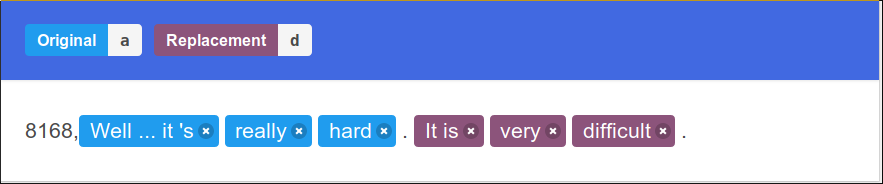
\includegraphics[width=\textwidth]{Figures/doccano.png}
    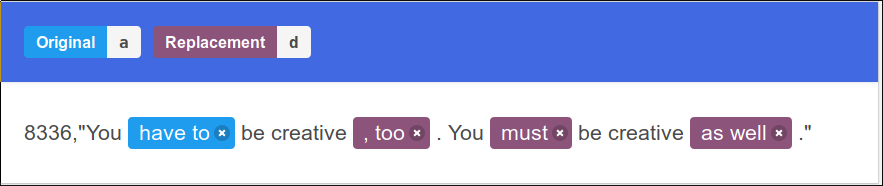
\includegraphics[width=\textwidth]{Figures/doccano2.png}
    \caption{Examples of how the sequence labeling annotation process looked using doccano.}
    \label{fig:doccano-ex}
\end{figure}

Finally, the segments had to be actually marked. I used a tool called \textbf{doccano} to carry out annotations on the paired informal blog post data and formal translated sentences (\cite{doccano2019}). Doccano's sequence labeling task annotator allowed me to select the spans of the sentences which were informal, and separately mark their formal translations. A couple of examples are displayed here at Figure \ref{fig:doccano-ex}. It is important to note that while multiple changes in the same sentences were able to be marked, this was only possible when the replacements were in the formal sentences in the same order that their original counterparts appeared in the source text. Additionally, some of the further syntactic movements were unable to be marked; however, as defined, this was in any case out of the range of the intended dataset, as the aim is to choose selected phrases to translate in-place.

\subsection{Final Characteristics}

Many of the sentences did not have annotations applied to them, either because the translated output did not change or because it changed in a way that no parallel phrases were available (for example, if the output quality was poor). In the end, there were 4848 phrases belonging to 3817 sentences (as some sentences were marked with more than one phrase).

The average Lexical Formality score for the Acrolinx data was calculated as $-0.15$, that is: informal, less informal than the GYAFC source data, more informal than the Microsoft source data and in fact approximately around the level of the Microsoft data when translated with the model from the previous chapter.

\section{Dataset Exploration}

Although the resulting dataset was small, it had the advantage of being human-validated in its entirety. Next, I present some examples from the set and results from testing and exploratory analysis.

\subsection{Examples}

\begin{table}[h]
\centering
 \begin{tabular}{|| p{6cm} | p{6cm} ||} 
 \hline
 Informal Phrase in Sentence & Formal Phrase in Sentence \\ [0.3ex] 
 \hline\hline
 Those lessons include : \textbf{don't} be afraid to chart your own course . & 
    Those lessons include : \textbf{do not} be afraid to chart your own course . \\
\hline
 That is why we are lucky enough to associate muffin tops with people 's waistlines , and to think of trolls not just as the mythological creatures that live under bridges , but also as the \textbf{guys and gals} who like to post mean-spirited comments online . & 
    That is why we are lucky enough to associate muffin tops with people 's waistlines , and to think of trolls not just as the mythological creatures that live under bridges , but also as the \textbf{people} who like to post mean-spirited comments online . \\
\hline
 \textbf{You can also} look at examples from other brands — competitors , or companies in other sectors — that might fire you up to stretch your tone a little bit . & 
    \textbf{It may be possible to} look at examples from other brands — competitors , or companies in other sectors — that might fire you up to stretch your tone a little bit . \\
\hline
 \textbf{And, if} you have been following along , you know that it is also inaccurate . & 
    \textbf{If} you have been following along , you know that it is also inaccurate . \\
\hline
 That may not seem like \textbf{such a big deal} , but the numbers quickly increase when you are referring to lots of different languages . & 
    That may not seem like \textbf{a big deal} , but the numbers quickly increase when you are referring to lots of different languages . \\
\hline
\end{tabular}
\caption{Examples from the resulting Acrolinx Blog Post Dataset.}
\label{acro-data-examples}
\end{table}

Some examples are given in Figure \ref{acro-data-examples}, formatted such that both marked phrases are given in the appropriate place of the original sentence. This also gives a sense of the original informality level of the texts --- casual, but certainly far less informal than the GYAFC data.

It is also clear that not every informal phrase in the original sentences has been identified and translated. Were one to write translations for the informal sentences individually, there are certainly other aspects that would be marked for change: perhaps ``fire you up'' to ``inspire you'', or ``lots of different languages'' to ``a variety of different languages'', as a start. Yet in a sense, this is a natural trade-off when switching from translating a whole sentence to locating and translating a phrase: the focus is to change the segments which can both have an effect on the overall formality of the sentence (make it \textit{less} formal) and have a low risk of scrambling the original meaning.

\subsection{Edit Categorization}

To get a better idea of what changes were covered in the new dataset, I examined the edits, again using doccano, and placed them each into one of eight potential categories. These categories included: when written-out phrases were changed to acronyms (\textbf{acronym}), written-out numbers replaced with digits (\textbf{number}), the removal of qualifiers/intensifiers as ``very'' and ``literally'' (\textbf{qualifier}), the removal of discourse markers like ``but'' and ``and'' (\textbf{discourse}), changing of punctuation (\textbf{punct}), grammatical or syntactic changes (\textbf{grammar}), the expanding of contractions into separate words (\textbf{contraction}), and the changing of words or lexical phrases with formal counterparts (\textbf{lexical}).

\begin{figure}
    \centering
    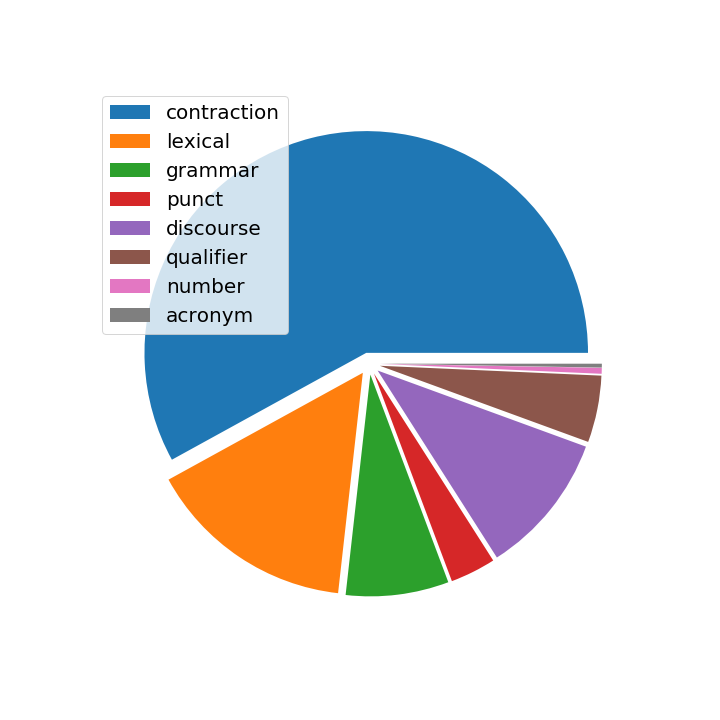
\includegraphics[width = 12cm]{Figures/pie_fig.png}
    \caption{Results of edit classification on the Acrolinx dataset.}
    \label{fig:doccano-edits}
\end{figure}

\begin{table}[h]
\centering
 \begin{tabular}{||c | r | l | l ||} 
 \hline
 Category & \% & Informal Example & Formal Example \\ [0.3ex] 
 \hline\hline
 contraction & 58.0\% & don't & do not \\ 
 \hline
 lexical & 15.2\% & plus & in addition \\
 \hline
 discourse & 10.4\% & So can you answer \textit{[...]} & Can you answer \textit{[...]} \\
 \hline
 grammar & 7.5\% & Go \textit{[...]} & You should go \textit{[...]} \\
 \hline
 qualifier & 4.9\% & absolutely agree & agree \\
 \hline
 punct & 3.3\% & \textit{[...]} with you! & \textit{[...]} with you. \\
 \hline
 number & 0.4\% & 13 & thirteen \\
 \hline
 acronym & 0.3\% & US & United States \\
 \hline
\end{tabular}
\caption{Percentages of each category of edit in the Acrolinx Blog Post Dataset, and examples.}
\label{acro-edits-table}
\end{table}

The results of this task are available in a visual sense in Figure \ref{fig:doccano-edits}, and with more specifics and examples in Table \ref{acro-edits-table}. As can be instantly seen, contractions make up the majority of the edits, likely because for the model which translated them, these were simple changes to pick up on and be consistent with. The changes in grammar were mostly the addition of relativizers or filling of technically incomplete sentences.

These figures are worthwhile to compare with those of Table \ref{pavlick2016table}, which gives the results from a similar effort by \cite{pavlick2016empirical}, due to the difference in domain. Though there is immediately visible overlap in the categories, there are also stark differences. As \cite{pavlick2016empirical} carried out their classification on changes in online debate forum data, there were other categories present that were not found in the Acrolinx blog posts: namely, \textit{normalization}, \textit{spelling} and \textit{capitalization} are examples of changes with, as they are considered linguistic errors, would not be present in professional texts like the Acrolinx blogs. Similarly, the punctuation changes are many more in their data as opposed to these data because the informality that using (for example) more than one exclamation mark brings is too high. The same applies to slang and idioms. That the two largest categories after capitalization and punctuation are ``paraphrase'' and ``delete fillers'', though, is analogous to the two largest after contraction for the Acrolinx data being lexical and discourse.

\section{Takeaway}

I confirmed that not all aspects of informality, as defined by \cite{pavlick2016empirical}, are present in the desired level of informality for this use case, as defined by these data from Acrolinx blog posts. Informality, as should by now be clear, takes on different sets of characteristics in different domains or contexts. With this in mind, I elected to narrow my focus for this project on those characteristics are most relevant and also approachable with machine learning techniques. Certain categories, such as expanding or creating contractions, are more likely to be achievable with rule-based methods. Others, which require deeper semantic understanding, could benefit from these algorithms.

From the selection gathered here, and for the presented reasons, I chose two categories of edits: discourse marker insertion and lexical/phrase replacement. Both had a significant presence in the Acrolinx data edits, and both necessitate understanding of their sentence- or even paragraph-level contexts.
\chapter{Discourse Marker Insertion}

\label{Chapter05}

\section{Problem}

Discourse markers are words or phrases which function to organize speech, by segmenting it, defining relationships between sections, and generally allowing a text to ``flow''. Despite their technically vague semantics and lack of a defined grammatical purpose (they can also be referred to as ``fillers''), they play an important linguistic part in both conversation and written speech.

As shown empirically both in this project (Table \ref{acro-edits-table}) and in previous literature (Table \ref{pavlick2016table}), discourse markers can be found in informal language, where they do not appear in formal language. A complete list of the discourse markers extracted from the informal side of the Acrolinx blog posts data is in Appendix \ref{Appendix01}. 

When entering a discussion on why these markers are present in informal language, it should be noted that the list in Appendix \ref{Appendix01} is not exhaustive. For example, ``nevertheless'', which is a discourse marker but certainly also formal, does not appear. Therefore, this problem inherently has a lexical component. Still, the definite and significant presence of at least these discourse markers in informal language invites these studies.

Discourse markers are likely regarded as informal in part because of their semantic vacuity: as discussed, formal language aims to be precise and absent of any so-called ``fuzzy'' terms. ``So there you have it'' --- where is ``there''? What is ``it''? Even with context, these things may not be immediately clear. The more surface-level, stylistic aspect of formality also comes into play here. In English grammar classes students are often prescriptively taught not to begin sentences with conjunctions, which would introduce a bias against discourse markers as ``but'' or ``and'' in speech that is meant to be more correct.

Following the pattern set by the edits categorized in the Acrolinx Blog Post Dataset, I focused on discourse markers which appear at the beginning of a sentence. This makes them easy to identify --- mid-sentence, some markers could be confused with other parts of speech, like ``now'' or ``first''. In any case, identifying and removing these markers from the beginnings of sentences is a fairly trivial task, perhaps able to be accomplished with lexicons alone. On the other hand, placing discourse markers in sentences is a different and certainly more difficult goal. ``But'' or ``so'' cannot be simply added to any sentence --- though the sentences can survive without them, they do signal an important relation between what has come before, and what is coming next. Even ``oh'', perhaps one of the simplest included markers, is interesting enough to inspire whole papers, and might signal some peripheral but still relevant information, or indicate an attempt to move a discussion forward (\cite{bolden2006oh}).

So, the insertion of discourse markers requires context, and both semantic and syntactic information. The resulting question to handle this problem became: given two consecutive sentences, can a particular discourse marker be inserted at the beginning of the second sentence? This gives both preceding and succeeding context to determine the potential presence of a marker.

I selected the most common nine discourse markers from the list in Appendix \ref{Appendix01}, based on the availability of data. Then, I trained a model for each of them to predict that marker's possible insertion in the sentence. Results were generally promising, though they seem to overpredict on out-of-domain data; increasing the softmax threshold works well in addressing this problem, though. In this chapter, I report on the data gathered, experiments developed and end results of this approach to the problem of (selective) discourse marker insertion.

\section{Data}

When compiling a dataset for this task, two main sources were used: the British National Corpus (BNC) (\cite{bnc}) \footnote{Data cited herein have been extracted from the British National Corpus, distributed by the University of Oxford on behalf of the BNC Consortium. All rights in the texts cited are reserved.} and the Open American National Corpus (\cite{ide2001oanc}). All texts were extracted and split into sentences. Only the texts from the OANC's spoken categories were skipped from then on, as they included no capitalization and included a high proportion of sentences of length 5 or less. 

\subsection{Sentence Pairs}

For each discourse marker, sentences in which that marker could be found at the start of the sentence (barring punctuation such as quotation marks) were extracted, along with the sentence preceding it. If there was no preceding sentence, the example was passed over; that context would be crucial to the experiment. I initially computed which discourse markers appeared most frequently in the data, and chose to focus on only those which had more than 1000 available samples.

Next, some special cases wherein the sentence could not stand without the discourse marker, or it was not a discourse marker at all, were removed. These included sentences that began with ``Now that'', ``First of all'' or ``So much that'', in which removing the word would have created a bad sentence. Pairs with sentences of length less than 3 were also removed.

Finally, the discourse markers were removed from the sentences, and the appropriate new first word capitalized in its place. A label was given to the sentence pair for the marker that was removed. If no discourse marker was present, the sentence pair was also given a corresponding label.

\begin{table}[h]
\centering
 \begin{tabular}{|| p{5.5cm} | p{5.5cm} | p{1cm} ||} 
 \hline
 First Sentence & Second Sentence & Label \\ [0.3ex] 
 \hline\hline
 Remember that scene in ``Sleeper'' where it's revealed that in the future everybody knows the only really healthy substances are red meat and cigarettes? & 
    Today's WP runs a story headlined ``Smoking May Protect Some High-Risk Women from Breast Cancer.'' &
    Well \\
\hline
 The paper points out that the episode is apt to rekindle consumer concerns about online credit card security. & 
    Since the jerkball's e-mail trail leads to eastern Europe, the case stands to highlight the freedom online criminals have to operate beyond U.S. jurisdiction. &
    Also \\
\hline
 In his shambling gait and glassy, uncertain stare he reminds me all too closely of another awesome wreck of a man who led another awesome wreck of a country: Marshall von Hindenburg at the end of his life. & 
    That scares me, because the similarities between Hindenburg's Weimar Germany and Yeltsin's Russia seem all too exact. &
    And \\
\hline
\end{tabular}
\caption{Examples of sentences with labels from the data compiled from the OANC and BNC.}
\label{disc-mark-data-examples}
\end{table}

The result was a dataset of tokenized sentence pairs, with discourse markers removed, and each one attached to a label of a specific marker or a label for no marker at all. A few examples are given in Table \ref{disc-mark-data-examples}.

\subsection{Vectorization}

I used doc2vec to vectorize each of the two sentences. Doc2vec trains an unsupervised model to learn feature representations of a predetermined length from variable-length text (\cite{le2014doc2vec}). I trained the model through a Python package called gensim (\cite{rehurek2010gensim}). With this method, not only can individual word information be encapsulated in output vectors, but syntactic relationships can also have an effect on the outcome.

I trained a doc2vec model on all sentences from the OANC and the BNC for 20 epochs, in order to produce 100-dimensional output vectors for each sentence. Final representation, therefore, was a sequence of two 100-dimensional doc2vec embeddings.

\subsection{Final Dataset Statistics}

\begin{table}[h]
\centering
 \begin{tabular}{|| l | r | r ||}
 \hline
 Data Subset & Number & \% \\ [0.3ex] 
 \hline\hline
 Total & 835,350 & --- \\
 \hline
 OANC & 273,702 & $32.8\%$ \\
 \hline
 BNC & 273,702 & $67.2\%$ \\
 \hline
 No Discourse Marker & 785,192 & $94.0\%$ \\
 \hline
 Discourse Marker & 50,158 & $6.0\%$ \\
 \hline
\end{tabular}
\caption{A numeric overview of the data on discourse markers compiled from the OANC and BNC corpora.}
\label{disc-mark-gen-data-stats}
\end{table}

Unsurprisingly, in the end there were far more examples without discourse markers in the original sentences than examples with them. An overview of the proportions of non-discourse marker sentence pairs versus sentence pairs with discourse markers removed, as well as how much data came from the BNC as opposed to the OANC, is presented in Table \ref{disc-mark-gen-data-stats}.

\begin{table}[h]
\centering
 \begin{tabular}{|| l | r ||}
 \hline
 Term & \# Examples \\ [0.3ex] 
 \hline\hline
 But & 21392 \\
 \hline
 And & 12918 \\
 \hline
 So & 4740 \\
 \hline
 Now & 2466 \\
 \hline
 Well & 2279 \\
 \hline
 Yet & 1909 \\
 \hline
 First & 1636 \\
 \hline
 Or & 1606 \\
 \hline
 Also & 1212 \\
 \hline
\end{tabular}
\caption{The number of examples for each removed discourse marker from the OANC/BNC data, from most to least.}
\label{disc-mark-dm-stats}
\end{table}

The original dataset was large enough that the resulting number of data points for each discourse marker were still substantial, particularly for the most common markers. The list of final chosen discourse markers to be used in these experiments, plus the number of samples labeled for each one, is given in Table \ref{disc-mark-dm-stats}. 

\section{Methods}

I trained a separate model for each discourse marker, on separate datasets extracted from the compilation described above. Therefore, the task was binary classification for each pair of sentences: could this discourse marker be inserted here, yes or no?

One could argue that a better methodology would be multi-class classification, wherein a single model predicts which of a list of discourse markers, if any, best fits between sentences. This was decided against for multiple reasons. Firstly, there is no reason why multiple discourse markers could not be a good fit for a given pair of sentences, if they share some contexts in which they are likely to appear (for example, ``and'' and ``also'', or ``now'' and ``so''). And secondly, the disparity in amount of data between discourse markers, as shown in Table \ref{disc-mark-dm-stats}, meant that creating a balanced dataset would either involve oversampling many times from the smaller terms, or subsampling from the terms with more data and thereby losing most of the potential samples. To encapsulate this potential of multiple discourse markers to appear in the same spot, and to fully take advantage of the terms which appeared more often in the data, I chose to train separate models.

\subsection{Architecture}

\begin{figure}
    \centering
    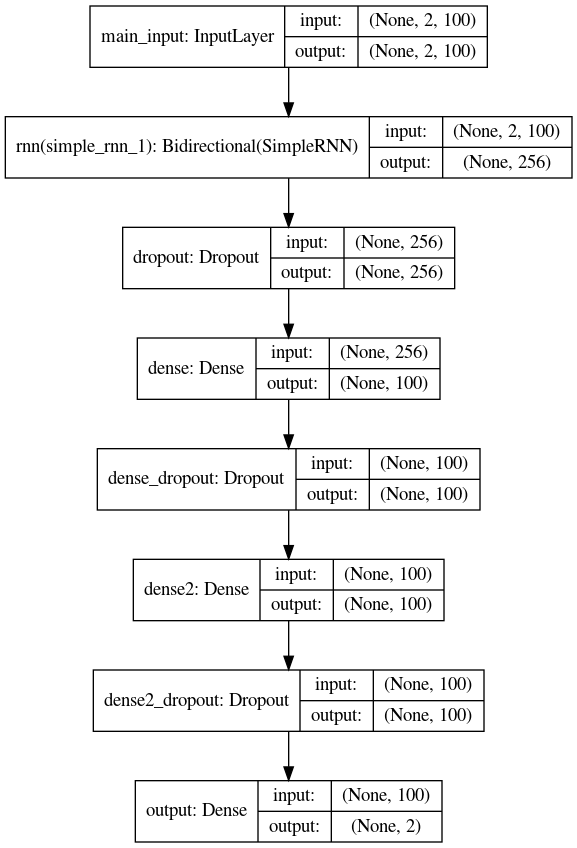
\includegraphics[width = 10cm]{Figures/graph.png}
    \caption{Visualization of the architecture for the models used to train for the discourse marker insertion task. Note that ``None'' represents the batch size.}
    \label{fig:disc-mark-architecture}
\end{figure}

The same architecture, developed using keras with tensorflow backend, was used to train all nine models (\cite{chollet2015keras}). It includes a bidirectional recurrent neural network (RNN) with 128 units followed by a dropout layer. After that there are two fully-connected layers with 100 units each and using rectified linear units (ReLU) for activation, each also connected to a dropout layer. Finally, there is a softmax output layer. The dropout rate is set to 0.5 for all relevant layers. Models are compiled with AdamOptimizer and the loss function is set to binary cross-entropy loss. A simple graph of the architecture with input and output shapes can be found in Figure \ref{fig:disc-mark-architecture}.

Hyperparameter optimization of the dropout rate and number of units for the RNN and the dense layers was carried out over the largest validation set, that of ``But'', and then kept constant for the models of the other discourse markers. The choice was made to not due individual hyperparameter optimization for each discourse marker due to the small dataset sizes of most of the others.

\subsection{Training}

\begin{table}[h]
\centering
 \begin{tabular}{|| l | r | r | r ||}
 \hline
 Term & train & val & test \\ [0.3ex] 
 \hline\hline
 But & 34655 & 3850 & 4278 \\
 \hline
 And & 20926 & 2325 & 2584 \\
 \hline
 So & 7678 & 853 & 948 \\
 \hline
 Now & 2995 & 443 & 493 \\
 \hline
 Well & 3690 & 410 & 456 \\
 \hline
 Yet & 3091 & 343 & 382 \\
 \hline
 First & 2650 & 294 & 327 \\
 \hline
 Or & 2601 & 289 & 381 \\
 \hline
 Also & 1963 & 218 & 242 \\
 \hline
\end{tabular}
\caption{The sizes of each training, validation and test set for the chosen discourse markers.}
\label{disc-mark-train-tune-test}
\end{table}

For each term, all the samples with the appropriate label were collected, and then a balanced dataset was compiled by randomly sampling the same number of instances from the data that had no discourse markers. Datasets were shuffled and then separated into train and test at a split of 0.9/0.1, and then the resulting training set was split into final train and validation at the same split of 0.9/0.1. This was done using the popular toolkit scikit-learn (\cite{scikit-learn}). Final lengths for training, validation and test sets are given in Table \ref{disc-mark-train-tune-test}. Some of these data subsets are quite small, and this should be kept in mind as we move on to look at results.

All models were trained for 5 epochs over their respective datasets with batch size 32. Training was very quick, with the largest set (``But'') taking only 8 seconds per epoch.

\section{Results}

Having nine different models with nine different dataset sizes means there are a substantial amount of numbers to keep track of. In this section I present quantitative results together with any overall trends or primary takeaways.

\subsection{Test Accuracy}

\begin{table}[h]
\centering
 \begin{tabular}{|| l | r | r | r | r ||}
 \hline
 Term & test-accuracy & precision & recall & f1-score \\ [0.3ex] 
 \hline\hline
 But & $76.5$ & $84.9$ & $64.2$ & $73.1$ \\
 \hline
 And & \color{red}{$78.6$} & $85.4$ & \color{red}{$70.8$} & \color{red}{$77.4$} \\
 \hline
 So & \color{red}{$77.1$} & \color{red}{$87.5$} & \color{blue}{$63.4$} & \color{red}{$73.5$} \\
 \hline
 Now & $75.5$ & $79.6$ & $65.0$ & $71.5$ \\
 \hline
 Well & \color{red}{$85.5$} & \color{red}{$91.9$} & \color{red}{$79.8$} & \color{red}{$85.5$} \\
 \hline
 Yet & $72.0$ & \color{blue}{$74.1$} & $66.7$ & \color{blue}{$70.2$} \\
 \hline
 First & \color{blue}{$69.4$} & \color{red}{$93.8$} & \color{blue}{$49.2$} & \color{blue}{$64.5$} \\
 \hline
 Or & \color{blue}{$70.7$} & \color{blue}{$67.2$} & \color{red}{$76.0$} & $71.3$ \\
 \hline
 Also & \color{blue}{$57.4$} & \color{blue}{$62.8$} & \color{blue}{$43.2$} & \color{blue}{$51.2$} \\
 \hline
\end{tabular}
\caption{Important evaluation metrics for the test sets, with the model trained for each term. The three highest scores for each metric are colored red; the three lowest are colored blue.}
\label{disc-mark-test-results}
\end{table}

The metrics used to evaluate the models were accuracy, precision, recall and f1-score. These metrics carried out on the test set for each model are given in Table \ref{disc-mark-test-results}. For each metric, the highest three scores are colored red, and the lowest three are colored blue. Overall, ``And'', ``So'' and ``Well'' had the best results, while ``First'', ``Or'' and ``Also'' performed the worst. Notably, all models except for that of ``Or'' had significantly better precision than recall. 

Note that the order the terms are presented in is preserved from Tables \ref{disc-mark-gen-data-stats} and \ref{disc-mark-data-examples}: descending order of dataset size. This provides additional context to our better- and worse-performing models: the models of those terms, which were trained on the least data (in all three cases less than 3000 training samples), struggled the most. This is likely to be an important reason for their performance.

\subsection{Training Accuracy}

\begin{table}[h]
\centering
 \begin{tabular}{|| l | r | r | r ||}
 \hline
 Term & train-during & train-after & validation \\ [0.3ex] 
 \hline\hline
 But & $75.0$ & \color{red}{$77.1$} & $76.2$ \\
 \hline
 And & $75.2$ & \color{red}{$78.9$} & $76.9$ \\
 \hline
 So & $72.2$ & \color{red}{$77.4$} & $75.6$ \\
 \hline
 Now & $66.8$ & \color{red}{$72.4$} & $67.1$ \\
 \hline
 Well & $81.6$ & \color{red}{$85.5$} & $84.7$ \\
 \hline
 Yet & $70.9$ & \color{red}{$74.6$} & $70.1$ \\
 \hline
 First & $70.5$ & \color{red}{$72.6$} & $70.8$ \\
 \hline
 Or & $74.1$ & \color{red}{$78.0$} & $75.2$ \\
 \hline
 Also & $63.1$ & \color{red}{$69.5$} & $66.2$ \\
 \hline
\end{tabular}
\caption{The resulting accuracy for the model of each term, over their training set while training happened (thus with dropout), and over both training and validation sets with the full number of units active. In all cases, the training accuracy given all active units is the highest (marked in red).}
\label{disc-mark-train-acc}
\end{table}

In this case, accuracy over the training set provides additional relevant information. In Table \ref{disc-mark-train-acc}, training and validation accuracy results are displayed. Two scores over the training set are actually given, the first, crucially, calculated during training, and the second in evaluation mode after training is over. For the most part, the accuracy results from during training are lower than the test accuracy results --- and this would be unexpected behavior for the model. However, this does not take into account that during training, accuracy is calculated by evaluating on the model with dropout. In the architecture presented here, with a dropout rate of 0.5, this could be a model with half of its units deactivated. The accuracy over the training set after training is complete is appreciably higher for all discourse markers. 

It should also be noted that this training accuracy and the test accuracy are fairly close in most cases. This suggests that the dropout rate has done its job of regularization: that the models were able to generalize to the test data. The only exceptions thereof are with the two models with the least data, ``Or'' and ``Also'', which performed significantly worse on the test data. These models were likely not able to generalize so well regardless of any regularization methods simply due to this lack of training information.

\section{Discussion}

Quantitative results alone cannot give us a good picture of what, exactly, the models are doing right and wrong. In this section I focus the discussion on error analysis, supported by qualitative data in the form of individual examples. In the interests of brevity, I will not go deep into the differences between the discourse markers, but will instead stick to overall patterns among them. 

\subsection{Noise in Negative Data}

The method of dataset collection here has left a problem. The data used to train these models was collected from real texts. The issue is that authors naturally do not always use these discourse markers where they \textit{could} be used. Therefore, while the positive samples (those which had the discourse marker originally) are definite cases of where the marker could go, the negative samples might have some data that are actually positive. A look at the negative training data confirms this:

\begin{quote}
\small{SENTENCE 1:} \quad The local authority served on the defendant written demands for the expenses they had incurred in respect of the works required under the notices, respectively on 31 May 1984 and 25 April 1985. \linebreak
\small{SENTENCE 2:} \quad \small{[NULL]} The defendant did not pay. 
\end{quote}

This was a negative sample for ``And''; however, ``And'' could still sensibly, perhaps even naturally, appear at the beginning of the second sentence. Interestingly, so could ``But'' --- further supporting the idea that while the two words might have opposing definitions as conjunctions, as discourse markers their differences are less clearly defined. Regardless, this form of noise in the data has two consequences: first, it would make it more difficult for models to learn what clearly separates a sentence which can take the marker from a sentence which cannot. Secondly, from what the model \textit{has} generalized, it may assign a positive label to a pair of sentences which could plausibly take the discourse marker, but which in the original data did not have it. 

Such is the case in the following example:

\begin{quote}
\small{SENTENCE 1:} \quad Their discord provided accompaniment for the chase that now developed between the two beings. \linebreak
\small{SENTENCE 2:} \quad \small{[true: NULL][pred: First]} She darted round and round the tower, running fast but waving her hands. 
\end{quote}

The original label was not ``First'', but the model predicted its presence. And in this case, ``First'' is a reasonable insertion for this pair of sentences.

Given this assumption of noise but only in the negative data, however, one might expect higher recall than precision. That is, the models, having generalized properly, would pick up not only all of the correctly labeled positive examples, but also all of the negative examples which could, in fact, take the discourse marker in question. Actually, though, the effects of the noise could be seen on precision and recall the other way, as well. The models may have also picked up in training on the improperly labeled negative data and thus tended to underpredict. It is difficult to separate out these two possibilities without having the entire dataset validated by humans.

\subsection{Lack of Context}

The other form of noise in the dataset has to do with the restricted context window. Two sentences were kept for each data point: the sentence which could have the discourse marker at its start, and the sentence immediately before it. This provides some context about the point the text is trying to make, the conversational place those sentences are at, and the logical progression of ideas. However, it naturally does not give all of that context. In some cases, these two sentences may not be enough. Consider:

\begin{quote}
\small{SENTENCE 1:} \quad I am glad that you talked to Ken Arrow.
\linebreak
\small{SENTENCE 2:} \quad \small{[true: But][pred: NULL]} Nobel laureates, who have wide responsibilities and much on their mind, are not necessarily on top of what has been going on in research outside their usual field.
\end{quote}

With these two sentences alone, one does not know anything about Ken Arrow, and what point the second sentence might be trying to make. Perhaps Ken Arrow is the busy and as such potentially uninformed Nobel laureate (for the record: he is), or perhaps a questioner failed to find their answer with another Nobel laureate, and then went to Ken Arrow for another opinion. Additional context could have made this placement more precise.

\subsection{Doc2Vec Issues}

The idea behind representing each sentence using doc2vec, instead of a sequence of word2vec embeddings, was that the syntactic and semantic information of each sentence would be contained in its vector. Then, when processing a series of sentences, the relationship between those sentences could be more clearly identified. Nevertheless, this method comes with its own disadvantages. Compressing, for example, a sequence of 20 word vectors, each with 100 dimensions, into a single 100-dimensional sentence vector, naturally means potential loss of important information --- particularly when that important information lies in a single word.

\begin{quote}
\small{SENTENCE 1:} \quad December is already an unkind month for those of us with combination skin .
\linebreak
\small{SENTENCE 2:} \quad \small{[true: But][pred: NULL]} On this third day of latkes, many of us awoke to find that our faces haven't been this splotchy since our bar mitzvahs.
\end{quote}

Whether or not ``But'' can be placed in this second sentence hinges on a single word in the first sentence: ``already''. With that word, placing that discourse marker is an option: this month is \textit{already} bad, and then something happened to make it \textit{worse}. Without it, though, the second sentence with ``But'' falls apart, as it then implies something nice about December should be coming, which is undoubtedly not the case. It is possibly the most important word for this problem in these sentences, and it may be that the doc2vec encoding causes its presence to be lost. Here is another example:

\begin{quote}
\small{SENTENCE 1:} \quad Quantitative methods were incorporated in the case study in two ways.
\linebreak
\small{SENTENCE 2:} \quad \small{[true: NULL][pred: First]} The first was in triangulation: the use of several forms of data within a single case study in order to give many reference points for verifying patterns and ruling out alternative explanations in order to achieve what evaluators call ``internal validity.''
\end{quote}

Here, there is a clear redundancy with the predicted insertion of ``First.'' If ``the first'' was not already there --- if, for example, it were replaced by ``one method was'' --- then the prediction would make sense. Instead of the overall semantic meaning and relationship of the sentences determining a prediction, it is both those overall characteristics \textit{and} the presence of a couple of important words which are most important. And again, when this (longer) sentence was transformed into a 100-dimensional vector, it is possible that a significant enough signal for the presence of those particular words was lost.

\subsection{Practical Usage: Microsoft Example}

Since an original problem with the GYAFC corpus and subsequent trained models was that it was too informal and did not translate well to out-of-domain data, specifically the Microsoft Azure corpus, it is helpful to try out these models on example text from those data. Ideally, when applying all these models to a text, key discourse markers would be suggested in certain places, helping the text to overall become more informal or conversational. Below is a sample passage from the corpus, with suggested insertions from all nine models given (\cite{microsoft2019azure}):

\begin{quote}
The Azure portal is a web-based, unified console that provides an alternative to command-line tools. \textbf{[Now/Also/And]} With the Azure portal, you can manage your Azure subscription using a graphical user interface. \textbf{[But/And]} You can build, manage, and monitor everything from simple web apps to complex cloud deployments, create custom dashboards for an organized view of resources, and configure accessibility options for the best experience. \textbf{[First/But/And]} The Azure portal is designed for resiliency and continuous availability. \textbf{[First/Now]} It has a presence in every Azure datacenter thereby making it resilient to individual datacenter failures and also avoids network slow-downs by being close to users. \textbf{[So/Also]} The Azure portal updates continuously and requires no downtime for maintenance activities.
\end{quote}

If these were suggestions to an author in order to make their text less formal, it might be too much. The models are overpredicting for this use case: there are too many suggestions, for too many of the sentences in a single paragraph. It is unhelpful as guidance for a writer.

Having softmax output gives us an easy way to tweak this, though. Often, the argmax function is used over the softmax output, meaning that if the probability of ``And'' being present is .51 and the probability of it not being present is .49, a positive prediction is given. By raising that threshold, one can ensure that the model predicts the positive class only when it has a higher degree of certainty as to its presence.

I raised the threshold to a probability of 0.75 to get the following output:

\begin{quote}
The Azure portal is a web-based, unified console that provides an alternative to command-line tools. \textbf{[And]} With the Azure portal, you can manage your Azure subscription using a graphical user interface. You can build, manage, and monitor everything from simple web apps to complex cloud deployments, create custom dashboards for an organized view of resources, and configure accessibility options for the best experience. \textbf{[And]} The Azure portal is designed for resiliency and continuous availability. It has a presence in every Azure datacenter thereby making it resilient to individual datacenter failures and also avoids network slow-downs by being close to users. \textbf{[So]} The Azure portal updates continuously and requires no downtime for maintenance activities.
\end{quote}

These predictions are fewer, more correct, and more concrete. They would provide more useful guidance to a writer who wants their text to be less formal.

\section{Future Work}

First and foremost, work could be done to clean any noise from the automatically gathered dataset. Manual validation would, naturally, be ideal. However, even if that is not possible, there are more steps that could be taken to reduce noise. For example, to compile negative samples for each model, instead of randomly sampling from the null case and all other discourse markers, one could sample only from the data for a discourse marker that tends to appear in different contexts. Examples might be ``But'' and ``First'', or ``Also'' and ``Or''. More research would be required to precisely delineate these patterns.

In general, more data from other corpora could be added, particularly for those discourse markers which had very small training sets. Given more data, it would be interesting to revisit the possibility of approaching this problem as a multi-class classification task, wherein the question becomes which discourse marker among a set could be placed in a particular sentence.

Next, more context could be added to the instances: instead of just a sentence pair, a series of sentences in a paragraph could all be vectorized to a sequence, with a mask to mark the potential location of the discourse marker. This could provide the necessary context to decide with more certainty if a certain marker can truly be inserted in a location, based on the overall content of the paragraph.

As discussed, doc2vec has advantages and disadvantages both. Directly comparing its usage with that of sequenced word vectors would provide useful insight and perhaps even turn out an improvement in performance.

And finally, other architectures could be experimented with. Transformers, which eschew recurrence entirely in favor of attention, could be a worthwhile avenue to explore for this task.

\section{Takeaway}

In general, this problem revealed itself to be trickier than it first seemed. There is ambiguity in many potential placements, and more context than expected turns out to be necessary in order to make precise predictions. Although the automatically formed dataset served its purpose well enough, future work would need to start with reducing its noise. 

Of course, in the end the purpose of attempting this task was to assist in the overall goal of making texts more informal. That brings us to the necessity of translating the question of ``Could this discourse marker go here?'' to ``Should an author add this discourse marker here, to make their text more informal?'' Adapting the models developed in this chapter to a practical usage would require further research. Nonetheless, results overall are promising, and could be extended for this purpose.
\chapter{Formal Phrase Replacement}

\label{Chapter06}

\section{Problem}

To change an entirely formal sentence to an entirely informal one could require, as seen in Section \ref{gyafc} about the GYAFC and Chapter \ref{Chapter03} about my work with that same dataset, complete transformation of a sentence, from syntactic structure to almost every individual word. Yet this comes with a risk of losing the meaning or fluency of the original sentence, and the level of informality could end up too high for the use cases relevant to this project.

In Chapter \ref{Chapter04} I found that when focusing on narrowing formality translation to the phrasal level, one of the largest categories of edits involved replacing certain formal words or phrases with corresponding informal ones (see Table \ref{acro-edits-table}). This was the second category that I chose as a task for this project: formal phrase replacement. That is, given a sentence, what phrase can be replaced with another to make the sentence more informal?

For this task I developed a two-part system, the first part of which locates the span containing a formal phrase in a sentence, and the second of which translates that segment to a less formal equivalent. Even moreso than the discourse marker insertion problem, this problem would ideally necessitate a large dataset manually validated by humans. Given that this was not possible within the scope of this work, the bulk of the work for this task was to automatically assemble a dataset as close to these ideals as possible, and focus on whether or not a model could be taught to generalize from these data.

% write something about the overall takeaway here

\section{Data}

The desired data format for this task is a sentence, a span marking the location of a formal phrase therein, and a phrase which could exactly replace that span and is also less formal than the original. This matches the format of the Acrolinx Blog Post Dataset. As there is not an existing dataset that fits this description --- the edits in the Acrolinx Blog Post Dataset which are in this category number only 441 --- one had to be compiled.

As an overview, the dataset was formed by taking a list of formal words and their informal replacements, finding each occurrence of each phrase in a collection of sentences, marking the larger phrases they were found in, and then replacing them within each phrase. I will detail the specifics of that process in this section.

\subsection{Initial Seed Words}

First, a set of seed formal words and phrases with informal replacements had to be gathered. Acrolinx, as described in Section \ref{acrolinx}, has existing lexicons with formal words and phrases, some of which already have suggested replacements. I gathered all of these terms, and those which had replacements were the original seed set. There were 258 terms and replacements in the original seed list.

\subsection{Phrase List Expansion}

The initial seed word list needed to be expanded to ensure a better variety of words and phrases, but not so much that it could not be manually validated in an efficient length of time. A list of potential expansion words started from the words in the Acrolinx lexicons that did not have informal replacements. Next, the Microsoft corpus was run through Acrolinx and the words that it marked as formal, according to the Lexical Formality score described in Section \ref{lf}, were also added to the potential expansion words. The subtask was the to extend the relationship between the paired words and phrases in the seed list to the potential additions.

To do this, I used word embeddings: specifically, a pretrained model from the developers of word2vec, which had vectors of 300 dimensions and was trained on the Google News corpus (\cite{mikolov2013word2vec}). Using simple vector math, one can create analogies of words. For example, consider the analogy: ``obtain'' is to ``get'', as ``purchase'' is to what word? By subtracting the vector for ``obtain'' from ``get'' and then adding the vector for ``purchase'', we find a point in the vector space. Looking at the words which are located closest to that point, we --- theoretically, as it does depend on the word embedding --- find the word ``buy''.

Thus, using this method for all the potential additions, the top 10 possible informal replacements for each term were collected. This method did mean that only single words were possible to add, and not whole phrases, as they do not have embedding vectors alone. As such, the list contains mostly single words and single word replacements, significantly more than it does phrases. From this, I looked over the list and kept only those words which were appropriate replacements, that kept the meaning intact while reducing formality. The edits from the Acrolinx blog post data were also added to this list.

Importantly, this meant that the final list sometimes offered more than one potential replacement word for any given formal word. Sometimes this was for grammatical reasons --- as ``commenced'' might require ``begun'' or ``began'', depending on the verb form --- and sometimes it was because there was more than one informal option.

One more manual verification step had to be completed before the list of formal words/phrases and informal replacements could be considered complete. I checked that each replacement could happen independent of context, or that in most contexts, at least one of the potential informal words or phrases could be inserted in the formal word or phrase's place.

The final list consisted of 827 formal phrases with informal replacements.

\subsection{Collected Sentences}

Similar to the discourse marker insertion approach, I took data from the British National Corpus and the Open American National Corpus (\cite{bnc}, \cite{ide2001oanc}). As this task did not require information at the paragraph level (which sentences come consecutively), I also added the sentences from the Brown corpus as provided through NLTK (\cite{bird2009nltk}, \cite{francis1979brown}). After removing items that were not actual sentences through preprocessing, the total number of sentences was approximately 3.8 million.

\subsection{Dataset Compilation}

Given the list of formal words/phrases and their informal replacements, it becomes simple with rule-based methods to simply identify those words and put any of the possible replacements in their place. However, this may not always be accurate, if there are multiple options for replacements not all of them may be appropriate for every context, and it would be restricted to only the words on the original list. With this task, the hope was to extrapolate beyond that, and to identify and translate other phrases.

Giving an informal replacement requires more than just a formal word, then: some context is needed. The collected list had some phrases, but mostly single words due to the use of word embeddings to expand it. On the other hand, giving the whole sentence only brings one back to the problem at the heart of this project: the risk of corrupting the meaning or grammar of the sentence. With that said, I chose to extract the syntactic phrases which the words were located in.

A package called spaCy was used to compute the dependency parse tree for each sentence (\cite{honnibal2017spacy}). If any formal words from the word list were found in the sentence, the nearest phrase in its dependency structure was marked as formal. More specifically: if it is in a noun phrase, then that phrase was marked. Otherwise, to ensure that a continuous segment was found, the nearest subtree was marked, looking first to the right and then to the left.

Marked locations are recorded in labels that match the sentence length, wherein each label is a binary indicator for whether or not its corresponding token belongs to a formal phrase.

\begin{table}[h]
\centering
 \begin{tabular}{|| p{8cm} | p{4cm} ||}
 \hline
 Sentence & Replacement \\ [0.3ex] 
 \hline\hline
 Her mother had taken great care \textbf{to provide a lot of love} and attention to Mary, often at the neglect of the baby. & to give a lot of love \\
 \hline
 Lose weight more quickly than ever before, because a larger proportion of \textbf{the calories you consume will remain} undigested. & the calories you consume will stay \\
 \hline
 This machine, \textbf{operating at speeds up to 350,000 revolutions per minute}, is believed \textbf{to provide one of the fastest} mechanical operations in industry today. & working at speeds up to 350,000 revolutions per minute \newline to give one of the fastest \\
 \hline
\end{tabular}
\caption{A few examples of sentences from the collected data for the Formal Phrase Replacement task. Marked formal phrases are in bold, with their replacements in the second column.}
\label{lexical-data-examples}
\end{table}

In the end, the dataset comprised 525,114 sentences from the three original corpora. With duplicates removed, the number of phrases with informal translations was 306,715. Some examples of sentences with marked formal phrases and their replacements are given in Table \ref{lexical-data-examples}.

\subsection{Vectorization}

For this task word2vec word embeddings were trained using gensim (\cite{mikolov2013word2vec}, \cite{rehurek2010gensim}). Vector dimension size was set to 100 with a context window of 5. Minimum number of appearances in the data in order to be counted in the vocabulary was also set to 5. The model was trained for 10 epochs over the entire set of sentences. In the end, the vocabulary size was a little under 150,000.

\subsection{Small Dataset}

A problem with the dataset was that phrases which included some words occurred far more often than others. Phrases centered around the word ``abaft'', for example, occurred less than five times, whereas ``thus'' was in thousands of sentences. To reduce the impact of this problem, and to see if overfitting to the phrase list could be preemptively avoided, a much smaller version of the dataset was compiled.

This time, when going through the sentences, if every formal word whose phrases were marked in the sentence occurred over 10 times in the dataset already, then it was not included. After this process the smaller dataset was complete at only 7146 sentences total.

\section{Methods}

As discussed, this task was split up into two models: one that would identify formal phrases in sentences, and a second that would take those formal phrases alone and translate them into informal equivalents.

\subsection{Phrase Identification}

\begin{figure}
    \centering
    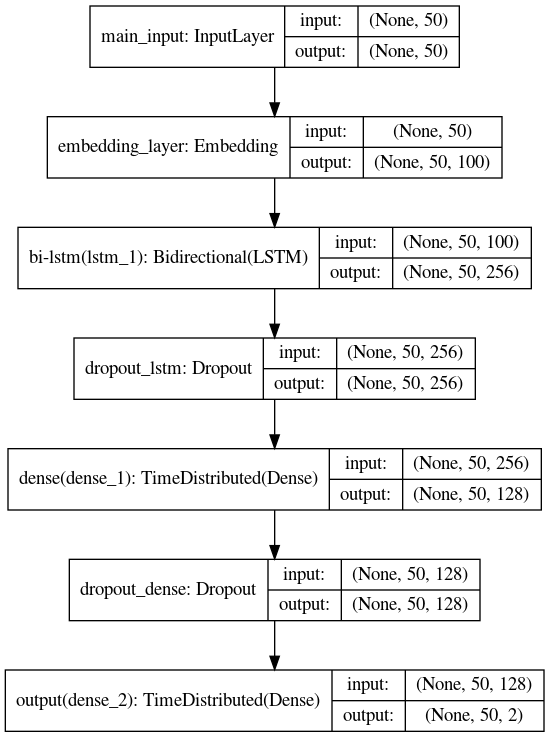
\includegraphics[width = 10cm]{Figures/graph-lexical.png}
    \caption{Visualization of the architecture for the models used to train for the formal phrase replacement task. Note that ``None'' represents the batch size.}
    \label{fig:lexical-architecture}
\end{figure}

A neural network was constructed for the task of finding the formal phrases within sentences. The maximum sentence length was set to 50; longer sentences were cut off and shorter sentences were zero-padded to that length. The architecture included a bidirectional LSTM with 128 units (each direction) and dropout (with a keep probability of 0.75), followed by a dense layer over the sequence with 128 units and dropout with rectified linear units as the activation function, and lastly a softmax output layer. A visualization of this architecture can be seen in Figure \ref{fig:lexical-architecture}.

The model was trained for one epoch over the entire dataset, which took about 45 minutes.

\subsubsection{Reduced Model}

Another model was trained on the small dataset, with some additional changes to the architecture. The number of units in the LSTM and dense layers was halved, so that it was 64. This was done, similar to the reasoning behind creating the small dataset in the first place, to reduce the capacity of the model to make it less likely to simply memorize the smaller amount of data. Otherwise, the architecture was the same. The model was trained for three epochs, which took altogether approximately three minutes.

\subsection{Phrase Replacement}

As the phrase replacement problem can be viewed a neural machine translation problem, only on the phrasal level instead of the typical sentential focus, I used OpenNMT for this part of the task (\cite{2017opennmt}). Default parameters were kept aside from the addition of copy attention, as before to allow the model to copy the parts of the phrase that should stay constant.

Training the model took about three hours, through 100,000 iterations. Notably, this was not even the full length of the dataset, but it was suspected that at that point more similar phrases would not have added any information to the model; furthermore, completing an epoch and doing a second run over the dataset might have enabled the model into memorizing the training set.

\subsubsection{Reduced Model}

Another model was trained that was identical to the ``main'' model, with the same OpenNMT parameters and training dataset, except instead of training for 100,000 iterations, it was only trained for 5000. Just like with the phrase identification model on the smaller dataset, this was meant to see if giving less information would make it less likely that the model only learns to replace the original word list instead of generalizing to other formal to informal translations.

\section{Results}

This section provides results for the main and the reduced models in order to compare them and evaluate how both models for both subtasks performed.

There were essentially two questions that needed to be asked in order to evaluate these models. First, did the models learn the initial list of formal phrases? This would be the baseline, what a rule-based formalism could accomplish: can the models identify and replace those words which were marked and translated in the dataset? To answer this question, results on the test datase in particular can be examined to see if a high degree of accuracy was achieved.

The second question is arguably more important, and it is: were the models able to move beyond the wordlist and generalize to other formal phrases and their informal translations? For this problem, the Microsoft data is used to see what else the models were able to learn.

% what did i find overall?

\subsection{Phrase Identification}

The first of our questions is addressed by evaluating results on the test and training sets.

\begin{table}[h]
\centering
 \begin{tabular}{|| l | r | r ||}
 \hline
 Term & train & test \\ [0.3ex] 
 \hline\hline
 Size & $472602$ & $52512$ \\
 \hline
 Accuracy (sentence level) & $69.2$ & $68.9$ \\
 \hline
 Accuracy (token level) & $97.6$ & $97.5$ \\
 \hline
 Precision (token level) & $86.8$ & $86.3$ \\
 \hline
 Recall (token level) & $88.6$ & $88.4$ \\
 \hline
 Avg errors per sentence & $1.22$ & $1.25$ \\
 \hline
\end{tabular}
\caption{Results for the phrase identification model which was trained on the full dataset. Accuracy at the sentence level is achieved if the model makes no errors over the full sentence.}
\label{phrase-ident-main-results}
\end{table}

Results are given in Table \ref{phrase-ident-main-results}. The default accuracy, at the token level, can be misleading, since the formal phrase(s) mark for the most part only a small portion of the sentence's length. Precision and recall help give a clearer perspective of the model's performance, but two other metrics were calculated in order to provide more information. One was accuracy at the sentence level, in which a sentence is considered correctly predicted if the label of every word has been predicted correctly. The other is the average number of incorrect labels per sentence.

These results show little overfitting (results on the train and test sets show only very small differences). While the numbers look impressive at first glance, this also suggests the opposite of what was desired: that the model did not generalize to phrases beyond the initial list used to assemble the dataset. If it had, the accuracy values, particularly for the test set, would be lower, as phrases which were not originally marked in the set would have been found and marked by the model.

\begin{table}[h]
\centering
 \begin{tabular}{|| l | r | r ||}
 \hline
 Term & train & test \\ [0.3ex] 
 \hline\hline
 Size & $6431$ & $715$ \\
 \hline
 Accuracy (sentence level) & $25.1$ & $21.7$ \\
 \hline
 Accuracy (token level) & $94.3$ & $92.7$ \\
 \hline
 Precision (token level) & $73.7$ & $62.4$ \\
 \hline
 Recall (token level) & $60.1$ & $55.6$ \\
 \hline
 Avg errors per sentence & $2.87$ & $3.65$ \\
 \hline
\end{tabular}
\caption{Results for the less complex phrase identification model which was trained on the reduced dataset. Accuracy at the sentence level is achieved if the model makes no errors over the full sentence.}
\label{lexical-ident-reduced-results}
\end{table}

For the reduced model, outcomes can be seen in Table \ref{lexical-ident-reduced-results}. As expected, results are worse across the board. Note in particular the large difference in sentence-level accuracy between this and the main model, as opposed to the small difference in token-level accuracy; the presence of the additional metrics makes it clear that this model did not learn as much as the previous. To clarify what exactly was learned and to answer the second of our questions, supplementary tests were run on the Microsoft corpus.

\subsubsection{Tests on Generalization}

\begin{table}[h]
\centering
 \begin{tabular}{|| l | r | r ||}
 \hline
  & Main & Reduced \\ [0.3ex] 
 \hline\hline
 Total Phrases Identified & $7093$ & $10197$ \\
 \hline
 Number of Generalized Phrases & $847$ & $4308$ \\
 \hline
 Percent Generalized Phrases & $11.9\%$ & $42.2\%$ \\
 \hline
\end{tabular}
\caption{Sentences from the Microsoft dataset were used as test data for both the main and reduced models for phrase identification, in understanding what the models were able to learn.}
\label{mic-phrase-ident}
\end{table}

10,000 sentences were randomly sampled from the Microsoft corpus for these tests, as to provide data for testing that is from a different source altogether from the training data. The purpose was to see, for both models, whether or not they were identifying phrases that went \textit{beyond} the initial word list used to create their training datasets. In the table, these are referred to as ``Generalized Phrases''. Results show that despite the constraints on the training data, both models were able to identify phrases which did not merely center around the wordlist. And as expected, the less powerful model trained on the reduced dataset picked up more than the full model.

\subsection{Phrase Replacement}

NMT approaches still present a difficulty with automatic evaluation; the case against BLEU for formality translation has already been presented in this report. This particular use, however, with its restricted scope, meant an easy method of evaluation presented itself.

\begin{table}[h]
\centering
 \begin{tabular}{|| l | r | r ||}
 \hline
  & 100k-iter & 5k-iter \\ [0.3ex] 
 \hline\hline
 Accuracy & $93.1$ & $91.5$ \\
 \hline
\end{tabular}
\caption{Binary accuracy results for the OpenNMT phrase replacement models.}
\label{phrase-repl-results}
\end{table}

To answer the first question --- has this model at least learned the word list? --- the output of the models on the test set was put to a simple test: was the word from the initial wordlist replaced within the original phrase, and all other words kept the same? The output of the 30,000 test sentence was used for this evaluation, and the results are given in Table \ref{phrase-repl-results}. The model trained on 5000 iterations was only slightly worse than the one trained on 100,000, showing that not much data at all was needed for the OpenNMT models to learn the initial word list.

\begin{table}[h]
\centering
 \begin{tabular}{|| l | r | r ||}
 \hline
  & 100k-iter & 5k-iter \\ [0.3ex] 
 \hline\hline
 Percent Changed & $43.4\%$ & $49.6\%$ \\
 \hline
\end{tabular}
\caption{How many phrases the translation models changed from the Microsoft formal phrases, as marked by the phrase identification systems.}
\label{phrase-repl-mic-test}
\end{table}

Next, the second question must be answered --- has this model gone beyond the word list? To address this, I collected the phrases marked as formal by both main and reduced phrase identification models on the Microsoft sample sentences. Skipping the phrases which only included one word, the final set contained 2010 phrases. The next check was to see if the input phrases were at all changed, or if the models simply copied them into the output. Although this does not evaluate whether or not any changes were sensible or not, the results of this basic test are included in Table \ref{phrase-repl-mic-test}.

An important caveat comes with these tests: it operates under an assumption that the phrases found by the phrase identification models in the previous part are correctly identified as formal, which may not be the case (in which case there would be nothing to translate, and the copying of the input to output would be a correct action). Still, the results do provide information. First, that the 5k-iter model changed more than the longer-trained model fits in line with the expectation that it had a reduced capacity for learning to only change the words from the initial list. Second, despite that observation, the difference between the two models is far less than that of the main and reduced phrase identification models. Similar to the accuracy results presented in Table \ref{phrase-repl-results}, this supports the finding that reducing the number of iterations to only 5000 did not make a huge difference. But without looking into the results qualitatively, as will be done in the next section, this alone is not enough to say that the models were able to generalize.

\section{Discussion}

In analyzing the results of the efforts for this task, there are two points to address, which conveniently correspond to the two questions focused on in providing results. The first of these concerns the small, but present error rate found when testing for the initial word list; the source of these mistakes should be examined. The second topic is regarding generalization, and entails honing in on what exactly the models have learned. Both of these topics are addressed for both subtasks here.

\subsection{Errors in Phrase Identification}

\begin{table}[h]
\centering
 \begin{tabular}{|| p{4cm} | p{4cm} | p{4cm} ||}
 \hline
 True Label & Main Model Output & Reduced Model Output \\ [0.3ex] 
 \hline\hline
 How is \textbf{the child's performance on the activity assessed}? & 
 How is the child's performance on \textbf{the activity assessed}? & 
 How is the child's performance on \textbf{the activity assessed}? \\
 \hline
 The footsteps went down, past the kitchen, into the shop; she thought they might vanish altogether but they shortly returned, \textbf{accompanied by a padding, clicking sound}, paws on linoleum. & 
 The footsteps went down, past the kitchen, into the shop; she thought they might vanish altogether but they shortly returned, \textbf{accompanied by a padding}, clicking sound, paws on linoleum. & 
 The footsteps went down, past the kitchen, into the shop; she thought they might vanish altogether but they shortly returned, \textbf{accompanied by a padding}, clicking sound, paws on linoleum. \\
 \hline
 But the Coroner says that for the time being\textbf{, Marc's death will remain a} mystery. & 
 But the Coroner says that for the time being\textbf{, Marc's death will remain a} mystery. & 
 But the Coroner says that for the time being, Marc's death \textbf{will remain a mystery}. \\
 \hline
 Does the ‘abc’ badge \textbf{provide any more comfort for the decision maker?} & 
 Does the ‘abc’ badge \textbf{provide any more comfort for the decision maker?} & 
 Does the ‘abc’ \textbf{badge provide any more comfort for the decision} maker \\
 \hline
\end{tabular}
\caption{Examples of errors made by the phrase identification models, in which they correctly identified the word from the initial list but did not match the phrase boundaries from the true label.}
\label{errors-phrase-ident}
\end{table}

As mentioned previously, the task of finding all words from a given list in a corpus should be a trivial one for a model. With that said, it would be curious that (as shown in Table \ref{phrase-ident-main-results}) accuracy at the sentence level was only 70\% for the main model. However, the task had been extended to find not only the formal words, but the phrases that contained them, so that at the next step, the context required to properly translate the word would be provided. In fact, most of the errors that the main and reduced phrase identification models made turned out to be differing placements of start and end boundaries for those phrases, wherein the main formal word was still included.

With the larger training set, it is unsurprising that the main model would pick up better on the syntactic rules (originally marked by spaCy's dependency parser) that were used to gather the data. The reduced model, while learning the words, does not seem to have achieved this goal to the same degree. Two examples where the reduced model did not match the true label but the main model did and two examples where both models misjudged boundaries are given in Table \ref{errors-phrase-ident}.

\subsection{Errors in Phrase Replacement}

\begin{table}[h]
\centering
 \begin{tabular}{|| p{4cm} | p{4cm} | p{4cm} ||}
 \hline
 source & target & pred \\ [0.3ex] 
 \hline\hline
 to \textbf{exclude} opinion evidence that sought & 
 to \textbf{keep out} opinion evidence that sought & 
 to \textbf{keep} opinion evidence that sought \\
 \hline
 to \textbf{ensure} that where the premises & 
 to \textbf{make sure} that where the premises & 
 to \textbf{make} that where the premises \\
 \hline
 to \textbf{determine} whether a payment made & 
 to \textbf{find out} whether a payment made & 
 to \textbf{find} whether a payment made \\
 \hline
\end{tabular}
\caption{Examples of errors made by the OpenNMT-trained phrase replacement models.}
\label{errors-phrase-repl}
\end{table}

With how stringently both phrase replacement models appeared to have memorized the initial list of formal words, even an accuracy of 90\% seems strange. An inspection of the predicted outputs reveals that most of the errors occurred when a multiple-word replacement for a single-word input was meant to happen. For example, instead of replacing ``ensure'' with ``make sure'', only ``make'' was added. A few examples of this phenomenon can be seen in Table \ref{errors-phrase-repl}.

Both the 100k-iter and 5k-iter models had this problem. It is possible that the inclination which the models learned to replace each word with a single-word replacement (as this was the case for the vast majority of examples) outweighed their memorization of the formal list.

\subsection{Generalization in Phrase Identification}

A problem with the results by the phrase identification models on the Microsoft sentences as shown in Table \ref{mic-phrase-ident} is that the category of ``Generalized Phrases'' would also contain most of the true errors made by the model. Since this category is automatically determined by checking if any words from the initial list appear in the phrase, improperly labeled phrases would also be put in it. This includes phrases which are actually not formal, a type of phrase difficult to discern without manual validation. It also includes cases in which the model ``split'' a phrase by, apparently randomly, marking a word within a formal phrase as informal, and causing it to be recognized as two separate phrases. Here is an example of this:

\begin{quote}
\textbf{The} JSON \textbf{structure that contains information about the conditions} when the start of speech was detected .
\end{quote}

In this case, ``The'' and ``structure that contains information about the conditions'' would be marked as two separate formal phrases. The above example is from the reduced model, which was more guilty of this error than the main model, particularly with unknown tokens such as ``JSON''.

\begin{table}[h]
\centering
 \begin{tabular}{|| p{5cm} | p{5cm} ||} 
 \hline
 Main Model & Reduced Model \\ [0.3ex] 
 \hline\hline
 key attestation & perform operations \\ 
 \hline
 the stored procedure & the incoming queries \\ 
 \hline
 asynchronous & these parameters \\ 
 \hline
 tabulated & evaluate the cost of your \\ 
 \hline
 expiry & if supported for some applications \\ 
 \hline
 recovery & inherited \\ 
 \hline
 log & predictive analytics \\ 
 \hline
 Remove the record & Linux \\ 
 \hline
 classifies the data that & concurrency control \\ 
 \hline
 proxy authentication using machine context & securing your PaaS web and mobile applications \\ 
 \hline
\end{tabular}
\caption{Some examples of phrases marked as formal by both phrase identification models on the Microsoft data.}
\label{phrase-ident-mic-examples}
\end{table}

Besides those errors, though, the formal phrases identified by both models do appear to be genuinely formal. In my observations, the reduced model performed better at still identifying whole phrases to provide some context for the next step. Some errors were certainly made (of this list alone ``log'' and ``Linux'' stick out as not particularly formal). With more work and tuning, the reduced model could better be able to identify formal phrases that it has never seen.

\subsection{Generalization in Phrase Replacement}

\begin{table}[h]
\centering
 \begin{tabular}{|| p{4cm} | p{4cm} | p{4cm} ||}
 \hline
 source & pred 100k-iter & pred 5k-iter \\ [0.3ex] 
 \hline\hline
 is not \textbf{deleted} & 
 is not \textbf{swapped} & 
 is not \textbf{left} \\
 \hline
 \textbf{define} the statement & 
 \textbf{show} the statement & 
 \textbf{describe} the statement \\
 \hline
 the \textbf{repository} & 
 the \textbf{field} & 
 the \textbf{replacement} \\
 \hline
\end{tabular}
\caption{Examples of output on the Microsoft formal phrases by the phrase replacement models.}
\label{general-phrase-repl}
\end{table}

Although the phrases from the Microsoft data were translated by the replacement models, a closer inspection of the output reveals that these translations are, optimistically put, misguided. A sampling of phrases is given in Table \ref{general-phrase-repl}. The patterns laid out here continue in the predicted data. The correct part of speech is maintained, and in terms of meaning, some vague idea seems to be preserved --- but, crucially, the only new words that both models provide are those which it learned to introduce in training.

One important thing to consider is that the default OpenNMT parameters were likely large enough that its capacity was too high for this task and dataset. A multi-layered encoder-decoder system with 500 units in each one, larger than any other model developed in this work, might have been more easily and quickly able to memorize the dataset, or at least only memorize the replacement words. This is something that will have to be more carefully tuned in the future.

\section{Future Work}

The primary task to continue with this research would be to better the dataset.

of course dataset stuff
backtranslation
hyperparameter optimization
if opennmt: mess with more parameters to make less powerful

\section{Takeaway}

% Chapter 1

\chapter{Conclusion} % Main chapter title

\label{Chapter07} % For referencing the chapter elsewhere, use \ref{Chapter1} 

\section{Main Section 1}

Lorem ipsum dolor sit amet, consectetur adipiscing elit, sed do eiusmod tempor incididunt ut labore et dolore magna aliqua. Ut enim ad minim veniam, quis nostrud exercitation ullamco laboris nisi ut aliquip ex ea commodo consequat. Duis aute irure dolor in reprehenderit in voluptate velit esse cillum dolore eu fugiat nulla pariatur. Excepteur sint occaecat cupidatat non proident, sunt in culpa qui officia deserunt mollit anim id est laborum.

%----------------------------------------------------------------------------------------
%	THESIS CONTENT - APPENDICES
%----------------------------------------------------------------------------------------

\appendix % Cue to tell LaTeX that the following "chapters" are Appendices

% Include the appendices of the thesis as separate files from the Appendices folder
% Uncomment the lines as you write the Appendices

\chapter{Additional Examples of Discourse Markers} 

\label{Appendix01} 

These are all phrases whose removal from informal to formal was categorized as an edit under ``discourse markers'', from the Acrolinx Blog Post Dataset.

\begin{enumerate}
  \item And
  \item So
  \item But
  \item Plus
  \item Now
  \item Or
  \item After all
  \item Sure
  \item Of course
  \item By the way
  \item Yet
  \item Okay
  \item Ok
  \item Well
  \item Again
  \item Since then
  \item Basically
  \item As such
  \item Oh
  \item Not only that
  \item As a result
  \item Anywho
  \item Anyhow
  \item Anyway
  \item Ah
  \item So there you have it
  \item Finally
  \item For starters
  \item At least
  \item Seriously
  \item In fact
  \item I'd argue
  \item You know
  \item You see
  \item I mean
  \item If so
  \item Beyond that
  \item Alas
  \item That way
  \item All told
  \item Yes
  \item Hey
  \item That's ok
  \item That's okay
  \item In fact
  \item That said
  \item With that said
  \item Uh
  \item Admittedly
  \item Unfortunately
  \item Fortunately
  \item First
  \item Recently
  \item Here goes...
  \item All told
  \item Heck
  \item In short
  \item First of all
  \item That is
  \item For example
  \item Also
\end{enumerate}
%\include{Appendices/AppendixB}
%\include{Appendices/AppendixC}

%----------------------------------------------------------------------------------------
%	BIBLIOGRAPHY
%----------------------------------------------------------------------------------------

\printbibliography[heading=bibintoc]

%----------------------------------------------------------------------------------------

\end{document}  
